
\documentclass[draft,linenumbers]{agujournal}
\draftfalse
\journalname{Journal of Advances in Modeling Earth Systems (JAMES)}
\begin{document}


\title{Implementing plant hydraulics in the Community Land Model, version 5}
\authors{Daniel Kennedy\affil{1},
Sean Swenson\affil{2},
Keith W. Oleson\affil{2},
David M. Lawrence\affil{2},
Rosie Fisher\affil{2},
Pierre Gentine\affil{1}
}


\affiliation{1}{Columbia University, New York, NY 10027 USA}
\affiliation{2}{National Center for Atmospheric Research, Table Mesa Drive, Boulder, Colorado, USA}
\correspondingauthor{Daniel Kennedy}{djk2120@columbia.edu}

\begin{keypoints}
\item An updated soil-plant-atmosphere continuum model based on hydraulic theory is implemented in the Community Land Model (version 5).
\item Prognostic leaf water potential replaces soil matric potential as the basis for stomatal conductance water stress. 
\item Prognostic root water potential is used to implement hydraulic root water uptake, replacing a `soil wilting point' approach.
\end{keypoints}



\begin{abstract}
Version 5 of the Community Land Model (CLM5) introduces the Plant Hydraulic Stress (PHS) configuration of vegetation water use, which is described and compared with the corresponding parameterization from CLM4.5.
PHS updates vegetation water stress and root water uptake to better reflect plant hydraulic theory.
The new configuration introduce prognostic vegetation water potential to the CLM, modeled at the root, stem, and leaf levels.
Leaf water potential replaces soil matric potential as the basis for stomatal conductance water stress, and
root water potential is used to implement hydraulic root water uptake, replacing a transpiration-partitioning heuristic function.
Point simulations of a tropical forest site (Caxiuan\~a, Brazil) under ambient conditions and partial precipitation throughfall exclusion are carried out to highlight the differences between PHS and the previous implementations of water stress and root water uptake.
Incorporating plant hydraulic theory advances the physical basis of the CLM, while creating a platform for testing hypotheses relating to the mechanisms governing vegetation water use dynamics within an Earth System Model.
\end{abstract}

%====================
%  INTRODUCTION
%====================

\section{Introduction}

Trees face emerging risk from climate change globally \citep{allen2010,anderegg2013b}, which may lead to increases in mortality and decreases in the terrestrial carbon sink.
In addition to stress from soil moisture drought, vegetation is susceptible to increasing atmospheric demand for evapotranspiration \citep{restaino2016,novick2016b,lemordant2018}.
Increases in vapor pressure deficit (VPD) are occurring with global warming \citep{ficklin2017,seager2015}, and are associated with impacts on vegetation, such as large-scale die-off \citep{williams2013,mcdowell2015}.
Understanding vegetation response to environmental drivers is important both for discerning future climate impacts on forests and for modeling feedbacks to the carbon and hydrological cycles \citep{lemordant2018}.
Significant uncertainty remains in Earth System Model (ESM) predictions of the carbon cycle, partly attributed to the response of vegetation to changes in hydroclimate \citep{dekauwe2017,friedlingstein2014,trugman2018}.

Soil moisture stress parameterizations are used by ESMs to determine the regulation of surface fluxes (photosynthesis, transpiration) by vegetation in response to water fluctuations \citep{egea2011,verhoef2014}.
Such parameterizations relate a metric of soil moisture status to leaf gas exchange, defining the response of stomatal conductance to declining soil water, serving to attenuate transpiration, photosynthesis, and root water uptake with drying.
Water stress dynamics have broad effects on critical land surface processes within models \citep{joetzjer2014}, such as evapotranspiration.
Likewise, because vegetation water use strategies modulate carbon uptake, creating a close coupling between the Earth System's carbon and hydrological cycles \citep{green2017}, vegetation water stress regulates the global carbon cycle.
This occurs on seasonal and interannual timescales, with stress attenuating transpiration \citep{dekauwe2015} and photosynthesis \citep{stocker2018}.
Furthermore, water stress parameterizations influence the diurnal cycle, through the partitioning of latent versus sensible heat, modifying the Bowen ratio \citep{gentine2007,gentine2011}. 
This in turn feeds back onto surface and air temperature, through land-atmosphere feedbacks \citep{bonan2008,seneviratne2006}.
Recent studies have shown that soil moisture stress functions are a major driver of uncertainty in leaf gas exchange in ESMs \citep{trugman2018} and can systematically overestimate the effect of soil moisture drought on evaporative fluxes \citep{ukkola2016,bonan2014}.
In Amazonia, which is the focus area of our model test runs, studies suggest that the CLM (version 3.5) simultaneously underestimates the effect of experimental drought treatment \citep{powell2013} and overestimates dry-season reductions in GPP \citep{restrepo2017}.

More mechanistic representations of stress and vegetation water use dynamics have been achieved by incorporating plant hydraulic theory into land surface models, modeling water flow throughout the Soil-Plant-Atmosphere continuum (SPAC)\citep{xu2016,christoffersen2016,sperry2017}.
Explicit modeling of water flow through the vegetation substrate increases model complexity, but is consistent with evidence of dynamic regulation of vegetation water use in response to both soil and atmospheric drying \citep{tardieu1998,sperry1998,sperry2015}.
Furthermore, because they are based on Darcy's Law, plant hydraulic models have a robust physical basis compared to models that utilize empirical water stress formulations.
Plant hydraulic models involve new parameters, which may prove challenging to constrain \citep{drake2017}, but plant hydraulic trait data are available \citep{kattge2011,anderegg2015a}, providing constraints on parameter estimation.   
Such trait data have been shown to improve predictions of species vulnerability to drought \citep{choat2012}.
Likewise vegetation water status observations are now available from remote sensing platforms, at a scale that is directly comparable to model development \citep{konings2016,grant2016} and therefore can be used to validate model results \citep{momen2017,konings2017b}.

In this study, we develop a new plant water stress parameterization based on hydraulic theory within the recently released Community Land Model, version 5 (CLM5, the land component of the Community Earth System Model, version 2). 
We refer to this hydraulics-based implementation as the `Plant Hydraulic Stress' (PHS) configuration. 
Previous versions of the CLM employed an empirical soil moisture stress function, as described above.


PHS, by explicitly representing plant hydraulics, introduces modeled vegetation water potential (discretized into leaf, stem and root elements) into the CLM, as well as a physical model of water supply, from the soil through the vegetation substrate. 
Transpiration is attenuated in the model according to leaf water status, capturing dynamic vegetation water use regulation in response to both soil moisture and atmospheric evaporative demand. 
These changes in the parameterization framework have numerous implications, including: 

\begin{enumerate}
\item Leaf water potential serves as a metric for plant water status instead of soil water or soil matric potential. As such, it reflects vegetation sensitivity to both soil and atmospheric drying, while serving as a diagnostic for excessive xylem tension and cavitation risk. 
\item Modeling plant hydrodynamics allows representation of hydraulic redistribution \citep{lee2005}, as the flow respects Darcy's law and thus is always directed down gradients of water potentials. 
\item Root water potential can be used to predict gradient-based root water uptake based on Darcy's law, replacing the previous empirical transpiration partitioning heuristic. This provides the means to vary, for example, the mean depth of extraction with changing soil water conditions.
\item Representation of a range of water use strategies (e.g. isohydricity and anisohydricity), improving the connection between plant carbon allocation and water availability.
\item Modeling vegetation water potential allows improved connection to remote sensing observations of vegetation water status (Vegetation Optical Depth) \citep{konings2016}. 
\end{enumerate}

To assess the new model formulation, we carried out site-level simulations at Caxiuan\~a National Forest in Brazil, which features a critical biome (terra-firme moist tropical evergreen forest) \citep{fisher2006}. Starting in 2001, a plot at this site was subjected to an approximately 50\% percent precipitation throughfall exclusion. Due to the large drop in soil moisture at the precipitation exclusion site, significant vegetation water stress regulation of transpiration and photosynthesis was observed at the site, providing a drought signal to demonstrate model dynamics \citep{fisher2007}.

In this paper we therefore:
\begin{enumerate}
\item Introduce the PHS theory and implementation in the CLM (Section 2)
\item Describe the details of the experiment setup (Section 3)
\item Analyze the dynamics of modeled water stress, root water uptake, transpiration, and soil moisture profiles (Section 4)
\item Discuss differences between PHS and the previous CLM water stress configuration (Section 5)
\item Outline the benefits and limitations of the new model (Section 5.7)
\end{enumerate}

%====================
%  MODEL DESCRIPTION
%====================
\section{Model Description}
This study uses CLM5 to compare two parameterizations of water stress (Sections \ref{sect:fwsms} and \ref{sect:fwphs}) and root water uptake (Sections \ref{sect:smsrwu} and \ref{sect:phsrwu}). The first parameterization, which we refer to as Soil Moisture Stress (SMS), deploys the CLM4.5 default root water uptake and water stress implementations within CLM5. The second is called Plant Hydraulic Stress (PHS); PHS is the default configuration of CLM5. In Sections \ref{sect:gs}-\ref{sect:wsf}, we describe the components that the two configurations share in common. In Sections \ref{sect:sms} and \ref{sect:phs}, we describe their differences.
    
    
%Photosynthesis
\subsection{Stomatal Conductance}
\label{sect:gs}
    CLM5 implements the Medlyn stomatal conductance model, which reconciles the empirical and optimal approaches to 
    stomatal conductance \citep{medlyn2011}.
    Such ``optimal'' stomatal conductance models serve to maximize photosynthesis relative to transpiration costs. 
    Stomatal conductance of water ($g_s$) is directly related to net photosynthesis ($A_n$) 
    and inversely related to the square root of the vapor pressure deficit near the leaf surface ($\sqrt{D}$) and the concentration of CO$_2$ at the leaf surface ($C_a$).
    \begin{equation}
    g_s=g_0+1.6\left(1+\dfrac{g_1}{\sqrt{D}}\right)\dfrac{A_n}{C_a}
    \end{equation}
    The model features two parameters: $g_0$ ($\mu$mol / m$^2$ / s) and $g_1$ (kPa$^{0.5}$). 
    The $g_0$ parameter is the minimum stomatal conductance, representing cuticular and epidermal losses (small). 
    The $g_1$ parameter relates to the marginal water cost guiding the optimization of carbon assimilation. 
    These parameters are plant functional type dependent.
    
    While maximizing assimilation relative to water transpiration costs, the Medlyn model does not 
    resolve concurrent limitations to stomatal conductance associated with declining soil water or excessive xylem tension. 
    To represent such water stress, and its impact on leaf-gas exchange, land surface models typically include a `water stress factor'. 

\subsection{Photosynthesis}
\label{sect:A}
    The CLM5 photosynthesis model is described in detail in \citet{bonan2011}, \citet{thornton2007},
    and \citet{oleson2013}. Photosynthesis is limited by three factors: carboxylation-limitations, light-limitations, and export-limitations 
    following \citet{farquhar1980} and \citet{harley1992}. Water stress (as discussed in the next section) is applied within the carboxylation-limited regime, by attenuating the maximum rate of carboxylation ($V_{\text{cmax}}$). The implementation extends \citet{sellers1996a,sellers1996b} with 
    co-limitation following \citet{collatz1991}. 
    
    The CLM5 photosynthesis module, in its default configuration, is a two-big-leaf model, with a sunlit and shaded leaf for each plant functional type \citep{thornton2007, dai2004, oleson2013}. 
    The canopy fluxes module iterates the solution for leaf temperatures to satisfy the leaf surface energy balances on both sunlit and shaded leaves, in response to forcing conditions.
    Within this, the photosynthesis module further iterates to solve for stomatal conductance and intercellular CO$_2$ concentration, balancing stomatal flux of CO$_2$ with photosynthetic assimilation flux of CO$_2$ (see Supp Fig B.1 for a flow chart of these iterations).


\subsection{Water stress factor}
\label{sect:wsf}
     Uncertainty remains within the literature as to how and where to apply water stress factors to photosynthesis and/or stomatal conductance 
    \citep{zhou2013,novick2016a,sperry2015}.
    In the CLM, the water stress factor ($f_w$) multiplies the `well-watered rate' of maximum carboxylation ($V_{\text{cmax,ww}}$) to effect water stress (as described in \citet{oleson2013}). 
    
    \begin{equation}
    V_{\text{cmax}} = f_w\, V_{\text{cmax,ww}} 
    \end{equation}

    Attenuating $V_{\text{cmax}}$ is not the only method for incorporating a response to declining water availability. 
    Other models opt to apply water stress directly to stomatal conductance, linking the stomatal conductance model slope parameter to soil moisture 
    (e.g. \cite{dekauwe2015}).
     However, \cite{lin2018} found that only the intercept parameter and photosynthesis (through changes in light-use efficiency) were sensitive to soil moisture based on eddy-covariance observations and not the slope parameter.
    Furthermore \cite{zhou2013} suggest that changes in assimilation tend to exceed those predicted by modulating $g_1$ with soil moisture, but could be captured by changing $V_{\text{cmax}}$. These results would thus suggest that it is appropriate to modulate $V_{\text{cmax}}$.
    Other field studies, however, suggest that measured $V_{\text{cmax}}$ at the leaf level does not change with drought \citep{flexas2004}. 
    On the other hand, the modeled $V_{\text{cmax}}$ is a bulk measure of $V_{\text{cmax}}$ and may implicitly account for mesophyll conductance changes \citep{rogers2017}, which has been shown to be water stress dependent \citep{flexas2012}.

    For now, applying water stress through $V_{\text{cmax}}$ seems well-supported, but future refinements may be appropriate.
    In this study, we preserve the method of applying water stress used in CLM4.5, while instead experimenting with how $f_w$ responds to environmental conditions.
    
    \subsection{SMS (CLM4.5 default)}
    \label{sect:sms}
    \subsubsection{SMS Water Stress Factor}
    \label{sect:fwsms}
    
    In SMS, the water stress $f_w$ is calculated as the summation of a soil layer wilting factor ($w_i$) across the $n$ soil layers, weighted by root fraction ($r_i$) \citep{oleson2013}.
    The soil wilting factor is a bounded linear function of soil matric potential ($\psi_{\text{soil},i}$).
    The function is defined by two parameters, the soil potential at (and above) which stomates are fully open ($\psi_o$) and the value at which stomates are fully closed ($\psi_c$).  

    \begin{linenomath*}
    \begin{equation}
     f_{w,\text{SMS}} = \sum_{i=1}^{n}{r_iw_i}
    \label{bt:1}
    \end{equation}
    \begin{equation} 
    \label{bt:2}
    w_i=0 \leq \dfrac{\psi_{\text{soil},i}-\psi_{c}}{\psi_{o}-\psi_{c}} \leq 1
    \end{equation}
    \end{linenomath*}
    
\subsubsection{SMS Root Water Uptake}
\label{sect:smsrwu}
    The CLM features a vertically discretized soil column with variable soil layer thicknesses.
    The number of soil layers ($n$) can vary, depending on the depth to bedrock.
    Soil water movement in each soil layer is governed by Richards' equation, with root water uptake ($q_i$) incorporated as a sink term.
    Summed over the soil column, root water uptake is required to equal transpiration ($T$).

    \begin{linenomath*}
    \begin{equation}
    T = \sum^n_i{q_i}
    \end{equation}
    \end{linenomath*} 
    
    In the SMS configuration, a heuristic function (based on $f_{w,\text{SMS}}$) is used to determine $q_i$.
    Transpiration is partitioned among the soil layers based on the product of the root fraction and the wilting factor, which is then normalized by $f_w$ to satisfy Equation 5.
    \begin{linenomath*}
    \begin{equation}
    \label{bt:4}
    q_i = \dfrac{r_i w_i}{f_w}T
    \end{equation}
    \end{linenomath*}
    
    Substituting for $w_i$ yields the SMS root water uptake equation as a function of the layer-$i$ soil potential ($\psi_{\text{soil},i}$).
    
    \begin{linenomath*}
    \begin{equation}
    q_i =
    \begin{cases}
    \label{eq:btrwu}
    0    & \text{if } \psi_{\text{soil},i}<\psi_{c}  \\
    \\[1pt]
        \dfrac{T}{f_w} \dfrac{r_i}{\psi_{o}-\psi_{c}} \left(\psi_{\text{soil},i}-\psi_{c} \right)     & \text{if } \psi_{c} \le \psi_{\text{soil},i} \le \psi_{o} \\
    \\[1pt]
    \dfrac{T}{f_w} r_i    & \text{if } \psi_{\text{soil},i} > \psi_{o}
    \end{cases}
    \end{equation}
    \end{linenomath*}
    
    In the Darcy framework, water fluxes are the product of hydraulic conductance ($k_i$) and hydraulic gradient ($\Delta\psi$).
    Although SMS does not explicitly calculate hydraulic conductance, Equation \ref{eq:btrwu} can be used to define hydraulic analogs resulting from the transpiration partitioning heuristic function, 
    allowing easier comparison to the PHS root water uptake implementation.
    
    \begin{linenomath*}
    \begin{equation} \begin{aligned}
    q_i &= -k_i\Delta\psi \\
    \Delta\psi &=  \psi_{c}-\psi_{\text{soil},i} \\
    k_i &= \dfrac{T}{f_w} \dfrac{r_i}{\psi_{o}-\psi_{c}} \\
    \mbox{constrained by:} \qquad
    \Delta\psi &=
    \begin{cases}
    0                          & \text{if } \psi_{\text{soil},i}<\psi_{c}  \\
    \psi_{c}-\psi_{o} & \text{if } \psi_{\text{soil},i}>\psi_{o}
    \label{kb}
    \end{cases}
    \end{aligned}\end{equation}
    \end{linenomath*}
    
    
   
% Plant Hydraulics
\subsection{PHS (CLM5 default)}
    \label{sect:phs}
    \subsubsection{PHS Water stress factor}
    \label{sect:fwphs}
    
    PHS introduces a new formulation of the water stress function, $f_w$, which is based on leaf water potential ($\psi_{\text{leaf}}$) instead of soil potential (described further in Section \ref{sect:demand}). The relationship is modeled with a sigmoidal function, subject to two parameters: the water potential at 50\% loss of stomatal conductance ($\psi_{50}$) and a shape-fitting parameter ($c_k$).
    
    \begin{linenomath*}
    \begin{equation}
    f_{w,\text{PHS}} = 2^{-\left(\dfrac{\psi_{\text{leaf}}}{\psi_{50}}\right)^{c_k}}
    \label{eq:fwphs}
    \end{equation}
    \end{linenomath*}
    
        \begin{linenomath*}
    \begin{equation}
\psi_{\text{leaf}} = \psi_{\text{soil}} + \Delta\psi
    \label{eq:fwphs}
    \end{equation}
    \end{linenomath*}
    
    Utilizing leaf water potential, instead of soil water potential, for drought stress introduces a new interpretation of vegetation water stress to the model. 
    Leaf water potential is modulated by supply of sap to the leaves and by evaporative demand, as regulated by stomatal dynamics \citep{novick2016a}. 
    As a result, low soil water (bottom-up stress) induces stress due to limited water supply, but in addition, high atmospheric VPD can induce stress with the associated increases in the gradient in water potential across the plant xylem (top-down stress). 
    This latter mechanism was absent from the previous water stress function (dependent on soil water potential only), by construction.
    Given the observed increase in VPD with global warming, it appears critical to include such mechanistic dependence of water stress.
    While the Medlyn stomatal conductance model does depend on VPD, the model does not (given constant $g_1$) reflect the risk of hydraulic failure \citep{zhou2013}.
    The new stress factor formulation reflects the dual risks of soil moisture deficit and atmospheric demand on hydraulic safety \citep{williams2013}, requiring vegetation to avoid excessive xylem tension associated with risk of cavitation.

    \subsubsection{PHS Root Water Uptake}
        \label{sect:phsrwu}
    
    PHS implements an alternative to the SMS heuristic approach for root water uptake, using a mechanistic representation following Darcy's Law.
    Instead of a constant parameter ($\psi_c$) defining $\Delta\psi$, PHS implements a physical model of vegetation water potential (described in Section \ref{sect:vwp}).
    The water flux from a given soil layer is driven by the gradient between soil potential ($\psi_{\text{soil},i}$) and the water potential in the root collar ($\psi_{\text{root}}$), 
    after accounting for the effects of gravity ($\rho g z_i$, where $z_i$ is the soil layer depth).
    Hydraulic conductance across the soil and roots ($k_{sr}$) is modeled based on soil hydraulic properties and xylem vulnerability, 
    accounting for both the path across the soil matrix and through the xylem conduits (details in Appendix B).
    
    \begin{linenomath*}
    \begin{equation}
        \begin{aligned}
    q_i &= -k_{sr,i}  \left(\psi_{\text{root}}-\psi_{\text{soil},i}+\rho g z_i\right)
    \label{phs:sink}
    \end{aligned}
    \end{equation}
    \end{linenomath*}

\subsubsection{Modeling Vegetation Water Potential}
\label{sect:vwp}
  The PHS model within CLM5 uses Darcy's law to model the flow of water through the SPAC, which can be represented with an electrical circuit analogy (Figure \ref{circuit}).
  PHS solves for vegetation water potential along the path from soil-to-atmosphere.
  Vegetation water supply and demand are both coupled to vegetation water potential, as described in the previous two sections.
  The solution for vegetation water potential is the set of values that matches supply with demand, maintaining water balance across each of the vegetation water potential nodes.

  \begin{figure}[h]
     \centering
     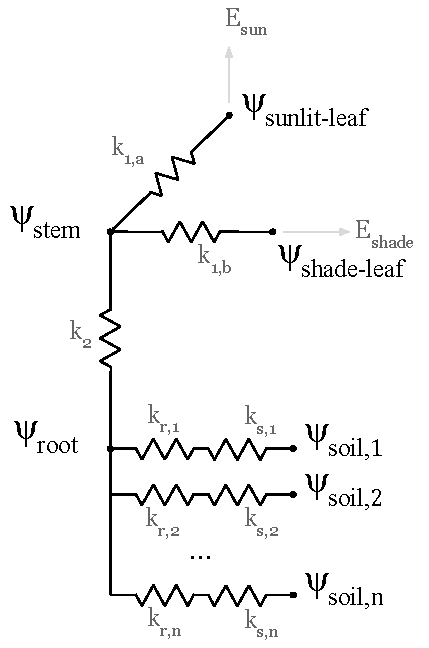
\includegraphics[width=9pc]{../figs/circuit.pdf}
     \caption{Plant hydraulic circuit analog schematic}
     \label{circuit}
  \end{figure}


  PHS solves for vegetation water potential at four locations: $\psi_{\text{root}}$, $\psi_{\text{stem}}$, $\psi_{\text{shade-leaf}}$, and $\psi_{\text{sun-leaf}}$.
  The number of nodes is chosen as the strict minimum to allow for differences in segment parameterizations \citep{simonin2015, sperry2015}, while also conforming to existing CLM model structure (vertically discretized soil layers, 2-big-leaf).
  At each node in the circuit diagram (Figure \ref{circuit}), we model water potential, and, between nodes, we resolve the flux of water based on Darcy's law. 
  Water uptake from the different soil layers is assumed to operate in parallel; a typical assumption justified by higher resistance in lateral versus central roots (e.g. \cite{williams2001}). 
  Two resistors operate in series between each $\psi_{\text{soil}}$ and $\psi_{\text{root}}$, to represent the path across the soil matrix and then through the root tissue \citep{williams1996}. 
  Specifics on the parameterization of hydraulic conductance for each segment are provided in Appendix B.1.
  Solving for vegetation water potential requires matching vegetation water supply (root water uptake, sap flux through the stem) with vegetation water demand (sunlit and shaded leaf transpiration).

   
%Water Supply
    \subsubsection{Water supply}
    \label{sect:supply}
    Water supply is modeled via Darcy's Law, where flux of water ($q$) is the product of the path hydraulic conductance ($k$) and the gradient in water potential ($\psi_2-\psi_1$) after accounting for gravitational potential ($\rho g \Delta z$).  
    Equation \ref{eq:darcy} represents the flow from a generic node 1 to node 2. 
    
     \begin{linenomath*}
     \begin{equation}
     \label{eq:darcy}
     q = -k\left(\psi_2 - \psi_1 + \rho g \Delta z\right)
     \end{equation}
     \end{linenomath*}
    
    For simplicity, PHS does not represent plant tissue water storage (or capacitance, using the electrical circuit analogy), which is in line with recent supply-loss theory \citep{sperry2015}.  
    Capacitance significantly complicates the water potential solution \citep{celia1990} and is challenging to parameterize \citep{bartlett2016}. 
    However, buffering of water stress provided by tissue water storage could potentially be important especially on sub-daily timescales \citep{meinzer2009,epila2017}, 
    whereby its inclusion may be warranted in future model versions.

     Hydraulic conductance through vegetation segments is modeled following empirical xylem vulnerability curves \citep{tyree1989}, where segments lose conductance with increasing xylem tension related to cavitation and embolism \citep{holbrook2001}.
      The vulnerability curves model loss of conductance relative to maximum conductance ($k_{\text{max}}$) using two parameters: 
      $c_k$, a sigmoidal shape-fitting parameter, and $p_{50}$, the water potential at 50\% loss of segment conductance (following \cite{gentine2016}). 
     
     \begin{linenomath*}
     \begin{equation}
     \label{eq:vulnerability}
     k = k_{\text{max}} \, 2^{-\left(\dfrac{\psi_1}{p_{50}}\right)^{c_k}}
     \end{equation}
     \end{linenomath*}
     
     Both $c_k$ and  $p_{50}$ can be estimated from field experiments \citep{sack2002}, and $p_{50}$ is available in the TRY trait database \citep{kattge2011}. 
     Parameterization based on $p_{50}$ aligns with the call for a transition to models that use a wider range of plant functional trait data in their parameterization \citep{anderegg2015a}. 
     The loss of xylem conductivity is based on lower terminal water potential ($\psi_1$) as is typical in other simplified models \citep{xu2016}, but 
     may underestimate the integrated loss of conductivity \citep{sperry2015}. 
         
     PHS models root, stem, and leaf tissue conductances according to equation \ref{eq:vulnerability}. 
     The parameterization of $k_{\text{max}}$ varies by hydraulic segment (see details in Appendix B1). 
     The conductances across the soil matrix ($k_{s,1}$,...,$k_{s,n}$) to the root surface follows \citet{williams2001} and \citet{bonan2014}, which scales
     soil conductivity \citep{brooks1964,clapp1978} by an appropriate conducting distance based on the root distribution.
     Details are provided in Appendix B1.
    
%Water demand
    \subsubsection{Water demand}
    \label{sect:demand}
    
    Water demand is calculated using the Medlyn stomatal conductance model (see Section \ref{sect:gs}) modulated by the CLM water stress factor.
    As discussed earlier $f_w$ is based on leaf water potential in PHS, where stress increases as leaf water potential becomes more negative \citep{klein2014}.
    Because leaf water potential is modeled separately for sunlit and shaded leaves, $f_w$ takes on distinct sunlit and shaded values.
    
     \begin{linenomath*}
     \begin{equation}
     \begin{aligned}
     \label{eq:d1}
     f_{w,sun} &= 2^{-\left(\dfrac{\psi_{\text{sun-leaf}}}{\psi_{50}}\right)^{c_k}} \\
     f_{w,shade} &= 2^{-\left(\dfrac{\psi_{\text{shade-leaf}}}{\psi_{50}}\right)^{c_k}}
     \end{aligned}     
     \end{equation}
     \end{linenomath*}
     
     Shaded and sunlit leaf transpiration ($E_{\text{sun}}$, $E_{\text{shade}}$) are calculated by attenuating maximal transpiration ($E_{\text{sun,max}}$,$E_{\text{shade,max}}$) according to $f_w$. 
     $E_{\text{sun,max}}$ and $E_{\text{shade,max}}$ are calculated at the beginning of each timestep by running the stomatal conductance model with $f_w=1$.
     Equations (\ref{eq:d1}) and (\ref{eq:d2}) reflect a simplification used within iterations of the PHS module, 
     neglecting non-linear components of the relationship between stress and transpiration (described further in Section zqz).
     
     \begin{linenomath*}
     \begin{equation}
     \begin{aligned}
     \label{eq:d2}
     E_{\text{sun}} & = f_wE_{\text{sun,max}} \\
     E_{\text{shade}} & = f_wE_{\text{shade,max}}
     \end{aligned}     
     \end{equation}
     \end{linenomath*}
     

 %PHS solution
    \subsubsection{PHS solution}
    \label{sect:solution}
    
    PHS solves for the set of vegetation water potential values ($\psi$) that matches water supply (root water uptake) to water demand (transpiration), while satisfying continuity across the four water flow segments (soil-to-root, root-to-stem, stem-to-leaf, and leaves-to-transpiration). 
    Beginning from an initial condition of $\psi$ (from the previous timestep), PHS computes the flux divergence $f$ (representing the mismatch of flow in and out of each segment) and iteratively updates $\psi$ until it reaches convergence, i.e. $f\to0$.
    
    \begin{linenomath*}
    \begin{equation} 
    \psi = \left[
    \begin{array}{c}
    \psi_{\text{sun}} \\ 
    \psi_{\text{shade}} \\ 
    \psi_{\text{stem}} \\ 
    \psi_{\text{root}}            
    \end{array} \right]
    \end{equation}
    \end{linenomath*}
    
    \begin{linenomath*}
    \begin{equation}
    f\left(\psi\right) = \left[ 
    \begin{array}{c}
    E_{sun}-q_{sun}\\
    E_{shade}-q_{shade}\\
    q_{sun}+q_{shade}-q_{stem}\\
    q_{stem}-\sum_{j=1}^n{q_{root,j}}
    \end{array} \right]
    \end{equation}
    \end{linenomath*}
    
    \begin{linenomath*}
    \begin{equation}
    A = \dfrac{df}{d\psi}
    \end{equation}
    \end{linenomath*}    
    
    While $\left|f\right|>0$
    \begin{linenomath*}
    \begin{equation} \begin{aligned}
    \label{eq:iter}
    \Delta\psi &=A^{-1}f\left(\psi_i\right) \\
    \psi_{i+1}  &= \psi_i + \Delta\psi
    \end{aligned} \end{equation}
    \end{linenomath*}    
    
    The numerics are tractable because $f$ has continuous, analytical derivatives and $A$ (a 4x4 matrix with six null entries) is easy to invert when well-conditioned. Supply and demand converge, because transpiration demand decreases with more negative leaf water potentials and supply increases with more negative leaf water potentials. The PHS loop is nested within iterations for intercellular CO$_2$ concentration and leaf temperature. The non-linear relationship between $f_w$ and transpiration is resolved through iteration for converging $f_w$ alongside intercellular CO$_2$. Details on the numerical implementation are provided in Appendix Section B.1.

 
%====================
%  EXP DESCRIPTION
%====================
\section{Experiment Description}
\label{sect:exp}

We use a set of four simulations to assess the impact of the plant hydrodynamics model (PHS versus SMS) on a tropical rainforest site, under ambient conditions and partial precipitation throughfall exclusion.
This site is located in Eastern Amazonia (Caxiuan\~a, Brazil) and part of the Large-Scale Biosphere-Atmosphere Experiment in the Amazon \citep{avissar2002}.

\begin{enumerate}
\item SMS, with ambient precipitation throughfall (AMB)
\item SMS, with 60\% of precipitation throughfall excluded (TFE)
\item PHS, AMB
\item PHS, TFE
\end{enumerate}

All four simulations use the same version of CLM5
(development version r270, www.github.com/ESCOMP/ctsm/releases/tag/clm4\textunderscore 5\textunderscore 18\textunderscore r270),
which features a switch that can toggle between SMS and PHS configurations.
Simulations are run offline (uncoupled from an active atmospheric model), spanning from 2001 through 2003, utilizing the satellite phenology (SP) mode of CLM5 in which vegetation state (LAI, canopy height) is prescribed and biogeochemistry is inactive. Six-year spin-up simulations (one each for SMS and PHS) are used to create initial conditions, repeating the Ambient simulation twice. Descriptions of site characteristics, forcing data, and observational sap flux and soil moisture, can be found in \cite{fisher2007} and \cite{fisher2008}.

\subsection{Parameter Values and Throughfall Exclusion}
\label{sect:param}
\begin{table}
\caption{Select parameter values}
\centering
\begin{tabular}{c c c c}
CLM name & Full Name & Symbol &  Value \\
\hline
kmax(1) & Maximum Sun Branch Conductance & $k_{\text{sun},\text{max}}$ &  4e-8 s$^{-1}$ \\
kmax(2) & Maximum Shade Branch Conductance & $k_{\text{shade},\text{max}}$ &  4e-8 s$^{-1}$ \\
kmax(3) & Maximum Stem Conductivity & $k_{\text{stem},\text{max}}$ &  4e-8 m/s \\
krmax & Maximum Root Conductivity & $k_{r,\text{max}}$ &  6e-9 m/s \\
psi50 & Water potential at 50\% loss of conductivity & $\psi_{50}$ &  -1.75 MPa \\
ck & Vulnerability shape parameter & $c_k$ &  2.95 \\
smpso & Soil potential with stomata fully open & $\psi_o$ & -0.65 MPa \\
smpsc & Soil potential with stomata fully closed & $\psi_c$ & -2.5 MPa \\
medlyn\textunderscore intercept & Medlyn intercept & $g_0$ &  100 $\mu$mol / m2 / s \\
medlyn\textunderscore slope & Medlyn slope & $g_1$ &  6 kPa$^{0.5}$ \\
n & Soil porosity to 4.64 meters & $n$ & 0.42 \\
n & Soil porosity beyond 4.64 meters & $n$ & 0.28 \\
hksat & Saturated soil hydraulic conductivity & $k_{\text{s,max}}$ & 3e-5 m/s \\
sucsat & Saturated soil matric potential & $\psi_{\text{sat}}$ & 461 Pa \\
bsw & Brooks-Corey parameter & $b$ & 6 \\
\hline
\end{tabular}
\end{table}

Parameter values concerning vegetation hydrodynamics are presented in Table 1. 
All other parameters use the default values associated with the r270 version of CLM5. 
Informed by parameter values reported in \cite{fisher2008}, we tuned soil hydraulic parameters and the throughfall exclusion rate, to improve simulated soil moisture relative to observations (Supp Fig \ref{supp:sm}).
A 972-member ensemble of simulations was used to tune the parameters for the PHS configuration to reasonably reflect sap flux observations (see Appendix \ref{ens}).


  \begin{figure}[h]
     \centering
     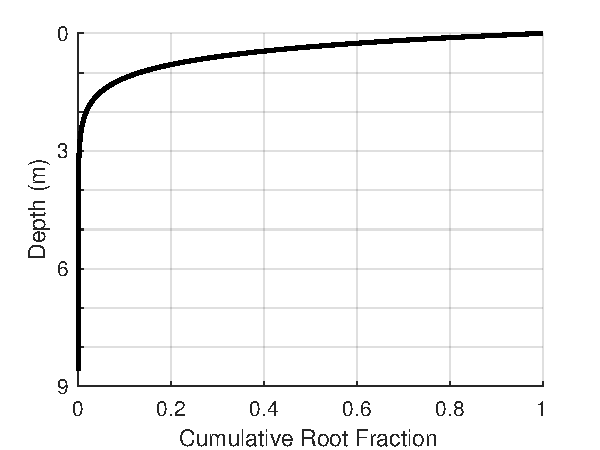
\includegraphics[width=20pc]{../figs3/roots.pdf}
     \caption{Cumulative rooting distribution. Likely moving to supplementary or cutting.}
     \label{roots}
  \end{figure}

%====================
%  RESULTS
%====================
\section{Results}  

\subsection{Comparison with observations}
\label{sect:obs}

We tested two configurations of CLM5 with simulations of the Caxiuan\~a throughfall exclusion experiment over 2001-2003. We compare modeled transpiration with observations derived from sap flux velocity and modeled soil moisture with observations using TDR sensors (see above for experiment and observation details).

\subsubsection{Transpiration, Ambient Conditions}
Under ambient conditions, PHS reduces error and improves correlation between modeled and observed transpiration (compared to SMS, Figure \ref{fig:t}a,c).
While the two models make a similar number of small errors, SMS commits more errors exceeding 1 mm/day.
The absolute value of SMS-OBS transpiration (Figure \ref{fig:t2}g) exceeds 1 mm/d in 67 of 414 days with available observations, as compared to just 23 with PHS.
And while PHS error is limited to a maximum of 1.6 mm/d, SMS error exceeds 2 mm/d twelve times (all of which underestimate transpiration relative to observations).
The largest SMS errors coincide with dry soils, which is discussed further in Section \ref{sect:smt}. 

While PHS offers improvements modeling transpiration as measured by RMSE and correlation, the ambient simulation seems to underestimate transpiration variability, with a standard deviation of daily transpiration of 0.61 mm/d compared to 0.87 mm/d in the observations (with SMS, the standard deviation is 0.97 mm/d).
As such, PHS features a low bias for high transpiration values and a high bias for low transpiration values (Figure \ref{fig:t}c).
The difference in modeled transpiration between PHS and SMS derives from divergent water stress dynamics, which are discussed in Section \ref{sect:stress}.

\subsubsection{Transpiration, TFE}
\label{sect:ttfe}
Both models demonstrate lower correlation and increased error relative to transpiration observations under TFE (Figure \ref{fig:t}b,d).
PHS performs better than SMS, but yields a more pronounced high bias (Figure \ref{fig:t}b,d).
The wet season (February-March-April), especially, is prone to high transpiration biases in both models, where, in the observations, transpiration is reduced 32\% by TFE, as compared to modeled reductions of only 1.6 and 4\% for PHS and SMS, respectively.
This may indicate that the models' sensitivity to soil potential declines are underestimated, or that water drains from the root zone more quickly after precipitation events than we represent in the TFE simulations (Figure \ref{fig:sm2}b,d).
Difficulty reproducing the effect of TFE (and the influence of soil moisture on leaf gas exchange) at Caxiuan\~a has precedent in the literature \citep{restrepo2017,powell2013}.

\subsubsection{Soil Moisture}
\label{results:sm}
The second source of observations for model evaluation is volumetric soil moisture. 
These data are used to evaluate the parameterization of root water uptake, which is updated with PHS.
Modeled soil moisture values (at a depth of 50 cm) are comparable between model configurations during the wet season (February-March-April) under ambient conditions, both yielding averages of 28\% (Figure \ref{fig:sm2}a,c).
With excess rainfall, soil moisture is largely determined by the soil field capacity and saturated conductivity, which are the same in both model configurations.
With water shortfalls, the root water uptake parameterizations drive the soil moisture dynamics, and the models diverge, 
as SMS consistently generates lower soil moisture values (than PHS) within the first meter of the soil column (Figure \ref{fig:sm2}, Supp Fig \ref{supp:sm2}).
Soil moisture averages to 10\% during the dry season (September-October-November, ambient case, depth=50cm) with SMS, as compared to 16\% with PHS.
PHS better comports with observations, reducing RMSE by 57\% relative to SMS (Figure \ref{fig:sm2}a,c).

We highlight the soil moisture at 50 cm depth, but similar patterns are observed throughout the first meter of the soil column (Supp Fig \ref{supp:sm2}).
The 50-cm depth emphasizes the effect of modeled root water uptake, because it features higher root fraction than the deeper soil layers (Figure \ref{roots}), 
but avoids the high frequency dynamics of the top soil layer from soil evaporation and precipitation events that do not relate to differences between PHS and SMS.
Under TFE, SMS minimum soil moisture is again limited to 10\%, but holds there for a longer duration (Figure \ref{fig:sm2}).
Contrastingly, PHS achieves lower dry season soil moisture values under TFE as compared to ambient conditions.
PHS better comports with observations, reducing RMSE by 42\% relative to SMS (Figure \ref{fig:sm2}a,c),
however both models seem to feature a high bias in soil moisture in the root-zone (under TFE) during the wet season (Figure \ref{fig:sm2}, Supp Fig \ref{supp:sm2}).

\subsection{Vegetation water potential}

PHS updates both the water stress and root water uptake parameterizations based on modeling vegetation water potential.
Leaf water potential features a pronounced diurnal cycle, reaching -1.65 MPa at midday (Figure \ref{fig:vwp}a).
Most of the midday pressure drop occurs between $\psi_{root}$ and $\psi_{stem}$ ($\Delta$=-1.47 MPa), representing the root collar and upper stem, respectively.
Stem, shade, and leaf curves are all roughly equal, resulting in overlapping lines in Figure \ref{fig:vwp}a, relating to high stem-to-leaf conductance from the parameter values used in this experiment.
Stem-to-leaf conductance does not drive leaf water potential in the current parameterization of the model, but may be important to investigate further, given the reported dynamics of leaf conductance \citep{simonin2015}. 
    
    Under TFE, model midday leaf water potential decreases to -2.31 MPa (Figure \ref{fig:vwp}b). 
    This change derives from a decrease in predawn root water potential (lower soil moisture) and in the drop in root water potential between predawn and midday (due to reduced soil-to-root conductance).
    This comports with previous evidence that seasonal changes in hydraulic resistance are larger belowground \citep{fisher2006}.
    Despite reduced stem conductance, the pressure drop from root-to-stem acts in the opposite direction, reduced in magnitude to -1.02 MPa (from -1.47 MPa), following from 54\% reductions in transpiration.
    In this way, stomatal regulation serves to mitigate the drop in leaf water potential due to soil drying and reduced hydraulic conductance. 

    Midday leaf water potential features a seasonal cycle, with lower values during the dry season (Figure \ref{fig:vwp}c).
    Under ambient conditions, modeled root water potential values comport well with wet season observations in \cite{fisher2006}, but are less negative than dry season observations.
    Modeled leaf water potential values under ambient conditions are less negative than field observations (\cite{fisher2006} report average $\psi_{leaf}$ of -1.71 MPa during the wet season and -2.47 MPa during the dry season), 
    but are within the range of observations.
    The parameter values used here may underestimate isohydricity (which would be reflected by minimal leaf water potential drop during drought) in response to TFE, given that observations showed no significant difference between ambient and TFE leaf water potential \citep{fisher2006}. 

\subsection{Stress dynamics}
    
    Modeling vegetation water potential enables a diurnal mode of variability in vegetation water stress.
    While the SMS stress factor has minimal diurnal variability,
    PHS features increased stress at midday (Figure \ref{fig:stress1}a,b), corresponding to the drop in leaf water potential induced by increasing demand for transpiration (Figure \ref{fig:vwp}b,c).
    Average midday stress values are comparable between the two model configurations during the 2003 dry season (Figure \ref{fig:stress1}), 
    but PHS achieves more photosynthesis over the course of the average dry-season day (Supp Fig \ref{supp:fpsn}), due to lower stress in the mornings and afternoons.
    
    The SMS stress factor lacks diurnal variability, because it is based on average root-zone soil matric potential (Equation \ref{bt:1}), which evolves over longer timescales.
    PHS utilizes leaf water potential to calculate stress (Equation \ref{eq:fwphs}), which responds to both water supply and transpiration demand.
    As such, the PHS stress factor responds to both soil moisture and VPD, while SMS responds only to soil moisture (Figure \ref{fig:stress2}).
    Under ambient conditions, SMS features significant stress associated with declining soil water status, but PHS stress is primarily demand-driven, with less impact from soil moisture (Figure \ref{fig:stress2}a,c).
    With TFE, stress increases in both model configurations, and the effect of soil moisture on PHS stress increases markedly (Figure \ref{fig:stress2}d).

\begin{table}
\caption{Root-zone soil potential $^a$ (MPa) terciles. The two cut-points are used to divide the points in each subplot of Figure \ref{fig:stress2} into three groups, based on root-zone soil moisture.}
\label{tab:tercile}
\centering
\begin{tabular}{c c c }
Simulation & T1 & T2 \\
\hline
SMS, Ambient & -0.01 & -0.54 \\
SMS, TFE & -0.29 & -1.74 \\
PHS, Ambient & -0.01 & -0.05 \\
PHS, TFE & -0.05 & -0.33 \\
\hline
\multicolumn{2}{p{.8\linewidth}}{$^{a}$SMS values correspond to daily mean root-fraction weighted soil potential.
PHS values correspond to predawn root water potential.}
\end{tabular}
\end{table}


\subsection{Gross primary productivity (GPP)}

The two stress parameterizations feature differing seasonal cycles of GPP, with PHS experiencing less seasonal variability in stress (Figure \ref{fig:gpp}a-d).
Under ambient conditions, SMS predicts little to no stress ($f_w$=1) during the wetter months (January through July).
Meanwhile PHS models significant stress, with highly variable $f_w$, ranging as low as 0.5.
Despite abundant soil water, PHS still imposes stress, due to high transpiration demand when VPD and downwelling solar radiation are high.
This results in lower wet season GPP than with SMS (Figure \ref{fig:gpp}e,g).
Contrastingly, SMS imposes more stress than PHS during the dry season (Figure \ref{fig:gpp}b,d), 
resulting in lower dry season GPP.
Observations show that GPP increases at Caxiuan\~a during the dry season \citep{restrepo2017}, suggesting that both model configurations, 
but especially SMS, may overestimate dry season water stress under ambient conditions.  

The modeled effect of TFE is relatively small during the wet season, with modeled reductions in GPP of 1.3 and 3.8\% for PHS and SMS, respectively.
Based on transpiration observations, both configurations likely underestimate the TFE effect during the wet season (discussed further in Section \ref{sect:stress}).
SMS imposes more dry season stress, resulting in a 63\% reduction of GPP due to TFE, compared to 44\% with PHS.
Comparing dry season stress to the wet season, and TFE conditions to ambient, precipitation shortfalls (and the associate reductions in soil moisture) lead to less added stress under PHS as compared to SMS.
However, PHS experiences more stress overall, due to the effects of xylem tension imposed by the gradient of water potential from soil-to-leaf (discussed further in Section \ref{sect:stress}).

\subsection{Root water uptake (RWU)}

In addition to updating water stress, PHS implements updated RWU, consistent with hydraulic theory \citep{cai2018,warren2015}.
The parameterization of RWU affects the vertical distribution of soil water (Figure \ref{fig:sm}, Supp Fig \ref{supp:sm}), as
SMS tends to achieve drier upper soil layers, whereas PHS spreads the drying effects of transpiration over a larger vertical extent.
As described in Section \ref{results:sm} (Figure \ref{fig:sm2}), this yields a dry bias relative to soil moisture observations in the root-zone for SMS (within the dry season).

RWU, within a given soil layer, is the product of hydraulic conductance ($k_{s,r}$) for water flow and the gradient ($\Delta\psi$) in water potential from $\psi_{\text{soil,i}}$ to $\psi_\text{root}$ (see Section \ref{sect:supply}).
With PHS, reductions in RWU with drying are imposed by declining $k_{s,r}$, which decreases by almost 3 orders of magnitude as soil potential declines from 0 to -1 MPa (Soil Layer 5, Supp Fig \ref{supp:cond}).
This derives primarily from the exponential dynamics of soil conductivity \citep{brooks1964}.
$\Delta\psi$ tends to increase with drying (due to dynamic $\psi_{\text{root}}$), partially mitigating the reductions to RWU imposed by $k_{s,r}$.
With SMS, the opposite is true: reductions in RWU are imposed by declining $\Delta\psi$ and are (to a small extent) mitigated by increases in the (implied) conductance. 
RWU (within a given soil layer) is more sensitive to soil potential with PHS (Figure \ref{fig:rwu}), which prevents soil potential from getting much lower than -1 MPa, as compared to values as low as -2.5MPa under SMS.

While RWU within a given soil layer is more sensitive to soil potential with PHS, transpiration overall is less sensitive to shortfalls in precipitation
associated with dry season onset and TFE (as compared to SMS, Figure \ref{fig:t2}).
This is because, within PHS, there is more flexibility to compensate for dry layers by switching the RWU to moist layers.
As such, PHS can compensate for its sensitivity to soil potential by spreading the drying associated with the transpiration sink over a larger vertical extent (Figure \ref{fig:sm}).
Following from this, with PHS, dry season transpiration is less sensitive to TFE, due to increased RWU from below 2 meters in depth (Figure \ref{fig:qdry}d).
The shifting of water extraction based on water availability is also present under ambient conditions, as PHS shifts RWU from near-surface (0-0.2m depth) to the deeper soil layers (beyond 0.2m) during drydowns (Figure \ref{fig:qdry}a-c).

Lastly, PHS eschews constraints on RWU imposed by SMS (Equation \ref{eq:btrwu}), that sets extraction to zero if $\psi_{\text{soil,i}}$ is drier than $\psi_c$ and to a maximal value when $\psi_{\text{soil,i}}$ is wetter than $\psi_o$ (SMS parameters for soil potential with stomates fully closed and open, respectively).
Hydraulic theory does not support either constraint.
Furthermore, the non-linearity of RWU at $\psi_c$ (Supp Fig \ref{supp:cond}), creates a situation where dry soil layers tend to stick at $\psi_{\text{soil,i}}$=$\psi_c$ (Figure \ref{fig:sm2}).
Likewise, the constraint at $\psi_c$ precludes the representation of hydraulic redistribution.

\subsection{Hydraulic redistribution (HR)}
    SMS precludes HR (contrary to PHS) setting root water uptake to zero when reversed gradients in water potential occur ($\psi_{\text{soil,i}}$<$\psi_c$).
    With PHS, HR totals to 38.9 cm under ambient conditions and 40.0 cm under TFE over the course of 2003, with the majority (28.0, 26.7 cm) of this HR occurring at night (Figure \ref{fig:hr}),
    in line with established theory \citep{jackson2000,lee2005} and observations \citep{oliveira2005,burgess1998}.
    HR occurs in both directions (Supp Fig \ref{supp:hr}), but is predominately downwards (AMB: 30.7cm, TFE: 33.8cm).
    The amount of HR is difficult to constrain due to scarce observations.
    The simplicity of the hydraulic representation may lead to overestimating HR, which is discussed further in Section zqz.

\subsection{Soil moisture effect on transpiration}    
    Model soil potential shows limited relationship to sap flux observations under ambient conditions (Supp Fig \ref{supp:cool}b,f), which is indicative of limited soil moisture stress.
    However, in the SMS configuration, modeled transpiration decreases strongly with more negative soil potential (Supp Fig \ref{supp:cool}a),
    biasing the model relative to observations (Fig \ref{fig:cool}a).
    
    Sap flux observations under TFE show a stronger relationship with soil potential especially with PHS (Supp Fig \ref{supp:cool}h,d).
    With SMS, the modeled attenuation of transpiration with soil potential again seems to bias modeled transpiration (Fig \ref{fig:cool}b).
    The two PHS simulations feature less structure in transpiration bias vs. soil potential and less bias overall (Fig \ref{fig:cool}c,d).
    
\section{Discussion}
\subsection{Can modeling vegetation water potential improve the CLM?}

    In this study, we have implemented plant hydraulic theory within CLM5, 
    using dynamic vegetation water potential to modulate leaf gas exchange and root water uptake.
    PHS installs a model for predicting vegetation water potential by extending Darcy's Law through the vegetation substrate (Figure \ref{circuit}), 
    creating four new water potential prognostic variables ($\psi_{\text{root}}$, $\psi_{\text{stem}}$, $\psi_{\text{shade-leaf}}$, and $\psi_{\text{sun-leaf}}$).  
    The model is able to capture expected diurnal and seasonal dynamics of vegetation water potential, 
    with lower values within the stem and leaves at midday and during the dry season (Figure \ref{fig:vwp}).
    PHS uses the new vegetation water potential variables to advance the physical basis for representing the SPAC, particularly with regard to modeling vegetation water stress and root water uptake.
    
    To demonstrate the new model dynamics, we utilized a site-level experiment testing PHS by simulating the Caxiuan\~a throughfall exclusion experiment \citep{fisher2007}.
    We found that PHS improves output for both transpiration and soil moisture relative to observations as compared to the control model (see Section \ref{sect:obs}, Figures \ref{fig:t},\ref{fig:sm2}).
    While this is encouraging, especially given the nature of the previous bias (see Section zqz), the improvement is specific to the site and experiment described herein, and model skill will need to be re-evaluated in a broader context.
    Instead, the value of opting for a single site (in lieu of global simulations) resides in the opportunity to perform the detailed analyses to elucidate the new model dynamics in order to complement this first description of PHS.
    

\subsection{Stomatal conductance: Soil moisture stress vs. Xylem tension stress}
    \label{sect:stress}
    
    The first of these analyses is of the response of stomatal conductance stress to environmental factors, namely: soil moisture, vapor pressure deficit, and solar radiation.
    The Medlyn stomatal conductance model, as implemented in the CLM, requires a notion of water stress to attenuate stomatal conductance in order to capture the effects of diminishing water supply,
    with various relevant implementations described in the literature (see Section zqz).
    We tested two such approaches, which alternatively base stress on either soil water potential (SMS) or leaf water potential (PHS).
    The two configurations feature significantly different stress dynamics on both diurnal and seasonal timescales (Figures \ref{fig:stress1},\ref{fig:gpp}).     
        
    Leaf water potential is (in simplified terms) the sum of soil water potential and the gradient of water potential from soil-to-leaf ($\psi_l=\psi_s+\Delta\psi$).
    Therefore using $\psi_l$ as the driver of water stress preserves a relationship between stress and soil potential, but now also represents the effect of increasing demand for transpiration (reflected by increases in $\Delta\psi$) on water stress, through increased xylem tension.
    As such, PHS offers a mechanistic approach to water stress, utilizing a physical justification that interprets water stress as the result of increasing xylem tension, which has previously been used as a primary \citep{sperry2017} or contributing \citep{novick2016a} factor to stomatal regulation.
    In the model, vegetation will (according to the specific hydraulic parameter values) limit transpiration in order to avoid cavitation and embolism associated with overly negative water potentials.
    As a result, PHS stress responds to changing soil moisture, but unlike SMS, also responds to VPD and downwelling solar radiation (Figure \ref{fig:stress2}), which modulate transpiration demand.
    This imparts a diurnal pattern to PHS stress, with higher stress around midday, whereas with SMS, stress is relatively constant throughout the day (Figure \ref{fig:stress1}).
   
    Soil water potential approaches (as in SMS) lack a straightforward physical basis, but rather empirically relate stomatal conductance and/or photosynthetic parameters with soil potential (or soil moisture).
    However, in the case of SMS, the empirical relationship is very difficult to constrain, due to scarce observations of the stress driver, root-fraction-weighted soil potential.
    As a result, soil moisture stress functions have been shown to contribute significant uncertainty to the carbon cycle in Earth System Models \citep{trugman2018}.
    Leaf water potential, on the other hand, is more easily measured in situ \citep{boyer1967}, and has been shown to correlate with remote sensing products \citep{momen2017}, offering better observational constraints for PHS.

    Another key difference is that PHS stress imparts a negative feedback on GPP and transpiration.
    Conditions favoring increased GPP (e.g. more light) also increase transpiration demand, leading to more xylem tension and stress, which opposes increases in GPP.
    In the PHS simulations, this suppresses variability in GPP relative to SMS, and leads to underestimating the range of transpiration compared to sap flux observations (Figure \ref{fig:t}).
    Terrestrial biosphere models have previously had difficulty reproducing variability observed in GPP \citep{keenan2012}, and evaluating the change in variability introduced by PHS will be an important follow-up to this study.
    With PHS, the relative contributions (to water stress) of changes in transpiration demand versus changes in soil potential (and likewise the strength of the negative feedback described above) can be varied by adjusting the hydraulic parameters. 
    This establishes a flexible representation of vegetation water use dynamics that can be used to test hypotheses about drought resilience, water use strategies, and the relative impacts of soil moisture and VPD on stress.
    
\subsection{Structural improvements in modeling root water uptake}

\subsubsection{Dynamic vegetation water potential}

PHS introduces dynamic vegetation water potential (Figure \ref{fig:vwp}), for the first time, into the default configuration of the CLM.
Seasonally and diurnally dynamic leaf water potential are observed in the field \citep{fisher2006}, adjusting to variations in soil water supply and transpiration demand.
Dynamism in the gradient of water potential from soil-to-leaf, according to Darcy's Law, drives RWU.
This is especially important for partitioning the transpiration sink among soil layers with varying soil potential states \citep{jarvis2011}.
A mechanistic representation of RWU with dynamic vegetation water potential allows for modeling a range of water use strategies, and/or testing hypotheses regarding such strategies on the ESM scale, including the effects of iso/anisohydry on leaf gas exchange and drought vulnerability.

\subsubsection{Mechanistic hydraulic conductance, with response to drying}
Likewise, PHS implements mechanistic hydraulic conductance through the SPAC, reflecting declines in conductance associated with decreasing water potential in both plant vessels and soil substrate \citep{tyree1989}.
Hydraulic theory describes soil conductance as featuring an exponential relationship with soil potential \citep{brooks1964}, ranging three orders of magnitude over the range of soil potential observed in our simulations (Supp Fig \ref{supp:cond}).
This shapes the PHS response of RWU to soil drought, and is not captured by the linear loss of RWU exhibited in SMS (between the parameters: $\psi_o$ and $\psi_c$, Figure \ref{fig:rwu}).
As a result, PHS RWU is more sensitive to drying soils, which seems to ameliorate dry biases in soil moisture observed in SMS relative to observations (Figure \ref{fig:sm2}).
At the same time, the mechanistic approach of PHS better reflects soil-root hydraulic theory \citep{cai2018,warren2015}.

\subsubsection{Compensatory RWU}
Utilizing a hydraulic approach (with dynamic vegetation water potential and mechanistic hydraulic conductance) enables a more flexible representation of RWU.
This includes the ability to model hydraulic redistribution (next Section) and compensatory RWU.
Compensatory RWU occurs when soil water extraction switches soil layers to maintain transpiration through precipitation shortfalls.
For example, as surface soil layers dry, tap roots can be used to harness reserves of soil water at depth \citep{oliveira2005}, partially compensating for reduced RWU near the surface.
In an SMS-style paradigm, this process is not represented \citep{jarvis2011}.

With identical rooting profiles, PHS extracts 29\% of transpiration from beyond 2 meters depth under TFE (during the 2003 dry season) as compared to 13\% with SMS.
In PHS, as the surface soil layers dry out, conductance decreases rapidly, leading to reduced near-surface RWU.
In response, the vegetation `pulls' harder, as $\psi_{\text{root}}$ becomes more negative, creating a larger gradient to the deeper soil layers, yielding increased RWU in those still-moist layers.
Due to constant vegetation potential ($\psi_c$) and no drying response to conductance, SMS lacks the flexibility to achieve this type of compensatory RWU.
As a result, PHS maintains higher levels of transpiration and photosynthesis than SMS during the dry season under both ambient and TFE conditions (Figures \ref{fig:t2},\ref{fig:gpp}).
This process may be especially important for modeling evapotranspiration in semi-arid ecosystems \citep{jarvis2011}.

\subsubsection{Hydraulic redistribution}
PHS simulates substantial HR at our test site, both upwards and downwards (Figure \ref{fig:hr}, Supp Fig \ref{supp:hr}), which conforms with field observations \citep{burgess1998,oliveira2005}.
    Modeled HR is weighted towards downward transfers, moving near-surface water from rain events deeper into the soil column and thus saving it for when it is most needed such as during the dry season.
    This would seem to convey an advantage to deep-rooted individuals, banking water for later use out of reach of shallow-rooted competitors.
    HR can offer significant water subsidies during dry periods \citep{jackson2000} and has been highlighted as an important missing feature in CLM \citep{lee2005}. 
    However, we should note that observations of HR are extremely difficult and rare, and the degree to which HR actually occurs in real-world systems remains unclear. 
    Unequivocal detection of HR involves the observation of reverse flow along transport roots, typically at rates close to the detection threshold of sap flow monitoring systems. 
    
    Installing a representation of HR was not a primary objective in the development of PHS.
    Rather it was the natural consequence of our simplified Darcy's Law implementation for root water uptake.
    However, it remains to be seen whether HR, as modeled in this implementation, is a feature or a liability.
    One challenge we faced was that in an initial implementation of PHS, HR seemed to oversupply the top layer of the soil column (spanning 0 to 2 cm below the ground surface) and thus significantly degraded modeled soil evaporation (not shown). 
    To remedy this problem, we set the hydraulic conductance to zero in the uppermost soil layer, disallowing any root water uptake there.
    
    PHS may overestimate HR, given the simplified root system architecture \citep{bouda2017} 
    and the lack of an explicit representation of fine-root cavitation \citep{kotowska2015}.
    In our simulations, HR increases annual total root water uptake by up to 52\% relative to transpiration alone (2003, TFE). 
    Other models, similar to the SMS paradigm, disallow HR by constraining root water uptake to be positive \citep{xu2016}.
    We view the PHS implementation of HR into the default versions of the CLM as a `null' hypothesis for the functioning of this process, and as a platform to allow further refinement from the plant hydraulics community. 
    Isotopologues of water could be used as a tool to further constrain this redistribution in the CLM in the future. 
    
\subsection{The influence of soil moisture on transpiration}
    \label{sect:smt}
    The stress effects of declining soil water potential seems to bias SMS predictions of transpiration relative to sap flux observations (Figure \ref{fig:cool}a,b).
    Under ambient conditions, soil water shows little relationship with sap flux observations with either model configuration (Supp Figure \ref{supp:cool}b,f),
    however SMS modeled transpiration decreases strongly in response to soil drying (Supp Figure \ref{supp:cool}a).
    This creates a bias where SMS underestimates transpiration during the drier soil conditions, 
    which is in line with \cite{bonan2014}, where the water stress factor was found to impose too much attenuation of transpiration (in CLM4.5).
    
    With PHS the transpiration bias does not seem to strongly depend on soil potential, while also featuring less bias overall (Figure \ref{fig:cool}c,d).
    Likewise PHS yields a stronger relationship than SMS between soil potential and sap flux observations during TFE (Figure \ref{supp:cool}d,h).
    While improvements modeling transpiration were expected with PHS (more parameters), it seems promising that the gains are associated with the reduction of a soil moisture induced bias.
    This could indicate that PHS better models the relationship between soil potential and water stress or the dynamics of soil potential itself (or a combination thereof).
    The reduction in bias introduced by the water stress function (especially as it depends on soil potential) represents a major development, given repeated calls to improve vegetation water stress in the next generation of terrestrial biosphere models \citep{powell2013,rogers2017,trugman2018}.

\subsection{Benefits and limitations of PHS}

\subsubsection{Benefits}

\begin{enumerate}
    \item Advances the physical basis of the CLM
        \begin{itemize}
        \item Mechanistic xylem tension stress replaces empirical soil moisture stress
        \item Root water uptake reflects established hydraulic theory
        \item More appropriate response of water availability to root abundance 
        \end{itemize}
    \item Improves modeled vegetation hydrodynamics
    	\begin{itemize}
	\item Better match to observations of soil moisture and transpiration (higher correlation, lower RMSE)
	\item Importantly, the improvements modeling transpiration are achieved by removing a bias associated with soil water status
	\item Permits representation of compensatory root water uptake and hydraulic redistribution
	\item Avoids excessive soil layer drying observed with SMS
	\end{itemize}
    \item Creates an interface to new observational constraints
        \begin{itemize}
        \item Parameters are better represented in trait databases (e.g. $k_{max}$, $p_{50}$).
        \item New state variables modeling vegetation water potential are introduced, which are measured in situ and are shown to correlate with remote sensing products
        \item And given that vegetation water potential is downstream of soil water potential, this may actually provide an important constraint on root-zone soil moisture.
        \end{itemize}
    \item Enables a platform for testing various hydraulics-oriented hypotheses within the ESM context
    \begin{itemize}
        \item What are the relative contributions to water stress of VPD vs. soil moisture?
        \item Does the spectrum of isohydric vs. anisohydric regulation of vegetation water potential explain patterns in the terrestrial carbon and hydrological cycles?
        \item Are certain regions of the concatenated hydraulic-parameter / climate space particularly vulnerable to climate change?
    \end{itemize}
\end{enumerate}

\subsubsection{Limitations}
\begin{enumerate}
    \item Plant hydraulics are highly simplified
    \begin{itemize}
        \item Does not model vegetation tissue water storage (capacitance)
        \item Loss of conductance (vulnerability) not integrated across vegetation tissue or soil matrix (based on lower terminus)
        \item Stem-to-leaf resistance is not fully deployed
        \item Simplified root system architecture
        \item These simplifications create a null hypothesis for further testing by the hydraulic community and yield a relatively light-weight model
    \end{itemize}
    \item Uncertainty regarding the parameterization of water stress
    \begin{itemize}
        \item PHS models water stress ($f_w$) as a sigmoidal function of leaf water potential, which is used to attenuate $V_{\text{cmax}}$
        \item Stress attenuation of $V_{\text{cmax}}$ was also utilized in CLM4.5/SMS, which allowed for easier comparison between model versions
        \item Several other approaches have been described in the literature, and future research is needed to elucidate water stress dynamics and mechanisms
    \end{itemize}
    \item Increased model complexity
    \begin{itemize}
    	\item Can potentially be mitigated by hydraulic trait coordination, improved parameter priors, and observational constraints on vegetation water potential
        \item However, the spatial scale of the CLM does not match to the experiments associated with reported parameter values in trait database 
    \end{itemize}
    \item We do not provide a definitive assessment on model skill
    \begin{itemize}
        \item Single site
        \item Results specific to experimental setup and parameter values
        \item However, this allows for more detailed analysis of the model dynamics to supplement the model description
    \end{itemize}
    
\end{enumerate}

\section{Conclusion}

    The PHS configuration of the CLM5 within the Community Earth System Model (CESM2) is, to our knowledge, the first land-surface model within an ESM with a representation of plant water potential running in its default configuration. In this paper, we have described the model implementation, and illustrated a comparison of the model dynamics for a tropical rainforest site subjected to water limitation, given that prediction of rainforest responses to drought is one of the key uncertainties in the ESM predictions \citep{huntingford2013}. Overall, the new model behavior differs from the default configuration in ways that are expected, given its structural properties, and in many cases, provides better correspondence with observations than the default structure. 
    
    In this paper, however, we have not aimed at undertaking a comprehensive assessment of which model structure performs better, given the substantial parametric uncertainty in both models, and the dependence on numerous other features of the CLM external to water stress representation that contribute to model-observation divergences - in this case in particular, the overestimation of unstressed transpiration by both versions of the model compared to the observations. 
    
    In lieu of this type of assessment, we propose that the new PHS model structure 1) is more closely aligned with known plant hydraulics theory, 2) provides significantly improved connections to real-world observational data streams (of leaf and stem water status, sap flow, percent loss conductance) and 3) represents known features of ecohydrological function that the default model cannot capture, including hydraulic redistribution, changes in the depth of water uptake with drought stress, plant embolism impacts on gas exchange, and responses of water uptake to changes in root abundance. 
      
\section{Acknowledgments}

\clearpage    

\section{Figures}

  \begin{figure}[h]
     \centering
     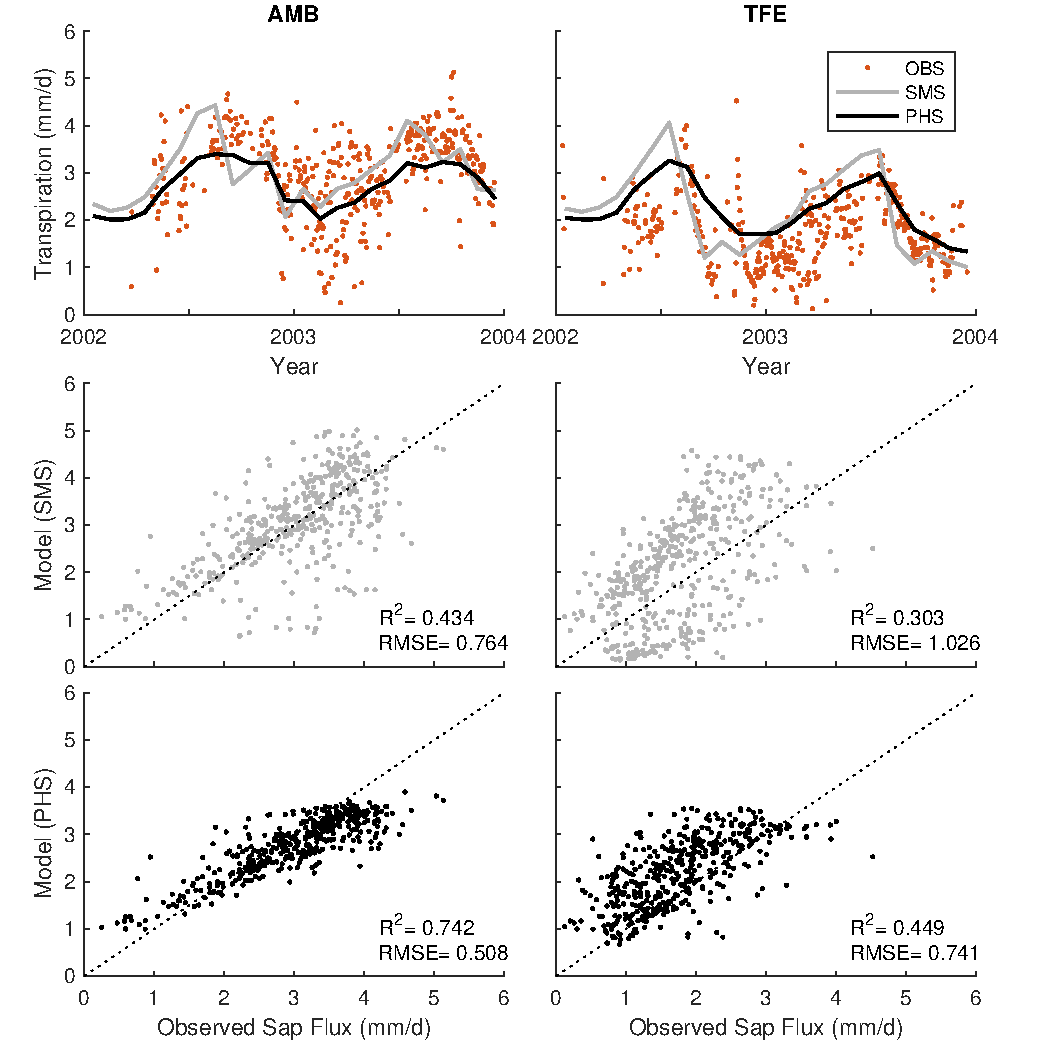
\includegraphics[width=30pc]{../figs3/T.pdf}
     \caption{Modeled versus observed daily total transpiration. Observations are derived from field observations of sap flux velocity (see Section \ref{sect:exp}).
     (a,b) SMS configuation, under ambient conditions and 60\% TFE.
     (c,d) PHS configuation, under ambient conditions and 60\% TFE.
     }
     \label{fig:t}
  \end{figure}
  
    \clearpage   
      \begin{figure}[h]
     \centering
     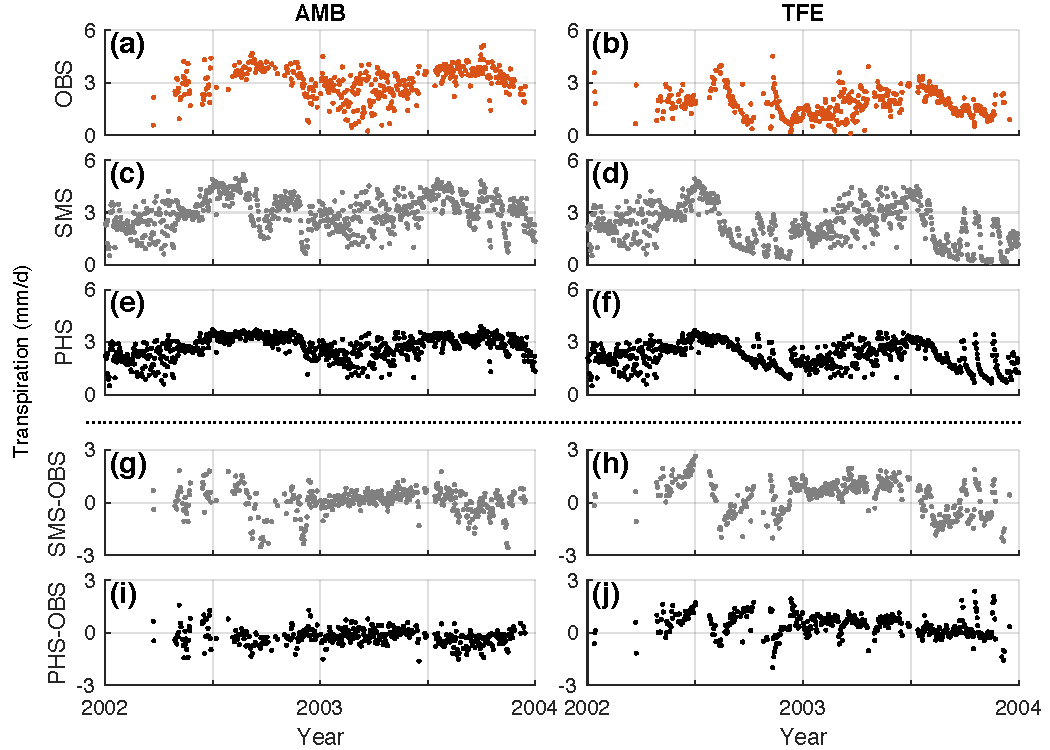
\includegraphics[width=30pc]{../figs3/fctr_ts.pdf}
     \caption{(a-f) Time-series of daily total transpiration (mm/d), from (a,b) observations, (c,d) SMS model configuration, and (e,f) PHS model configuration under ambient and TFE conditions.
     
     (g-j) Difference between modeled and observed transpiration (mm/d), for (g,h) SMS and (i,j) PHS under ambient and TFE conditions.
     }
     \label{fig:t2}
  \end{figure}
    


        \clearpage
    \begin{figure}[h]
     \centering
     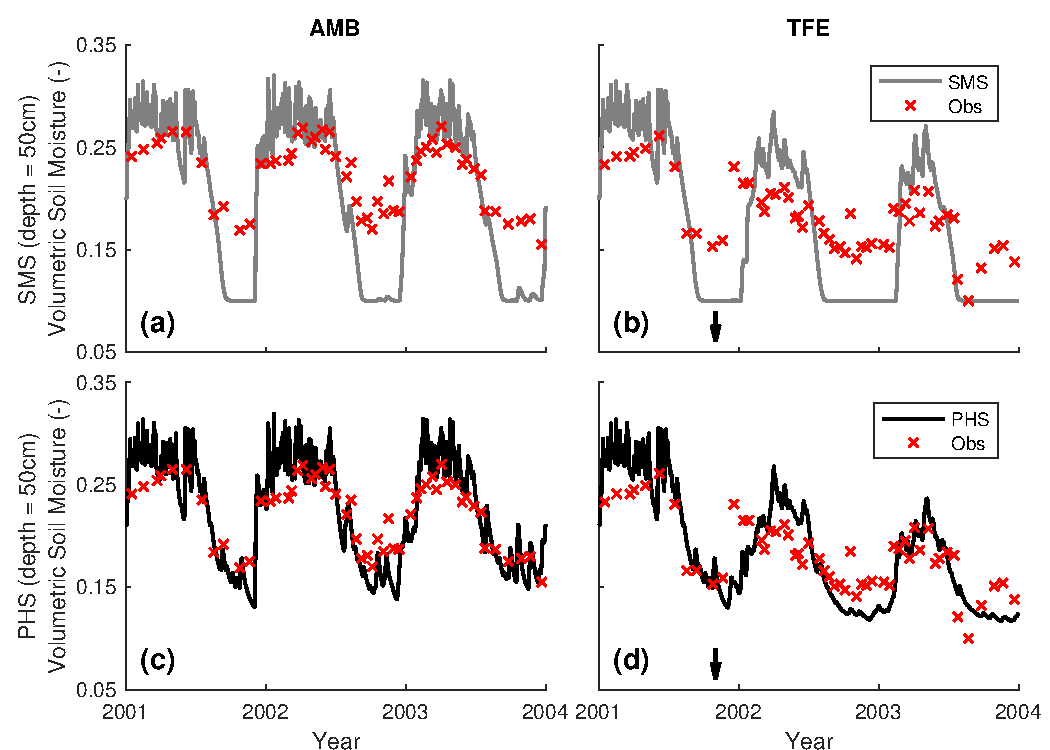
\includegraphics[width=30pc]{../figs3/sm2.pdf}
     \caption{Volumetric soil water content (-) over time under ambient and TFE conditions at a depth of 50cm.
     (a/b) SMS
     (c/d) PHS.
     Arrows indicate start of TFE. Figure \ref{supp:sm2} plots 7 other soil depths. Note that SMS can tend to `stick' at water content of 0.1 during the dry season, which corresponds to $\psi_{\text{soil}}$=-2.5MPa and is the value of SMS parameter $\psi_c$. }
     \label{fig:sm2}
  \end{figure}
  
  
    \begin{figure}[h]
     \centering
     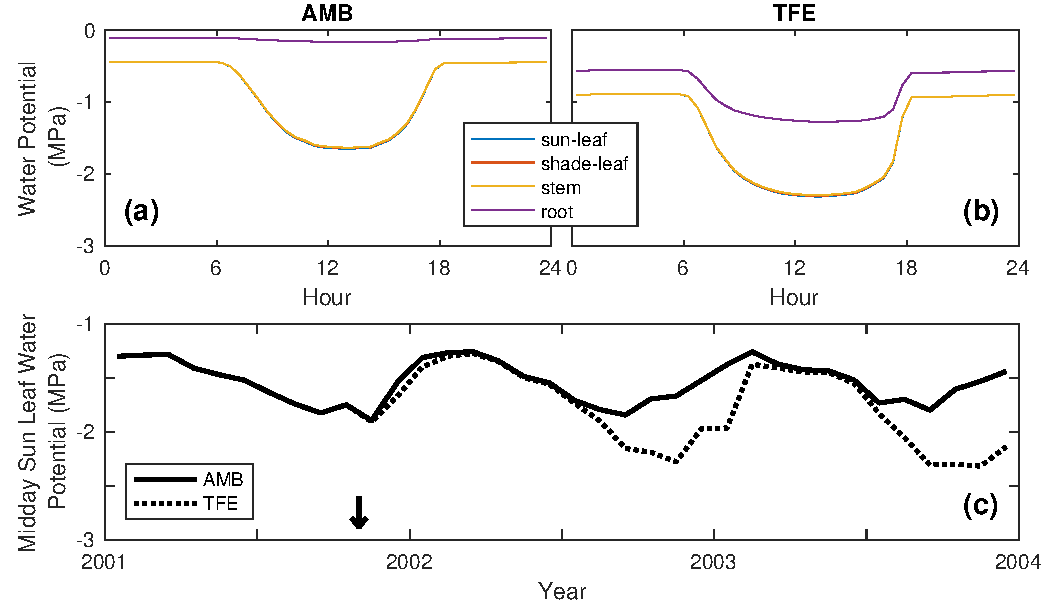
\includegraphics[width=30pc]{../figs3/vwp.pdf}
     \caption{(a,b) 2003 dry season (September-October-November) diurnal mean of modeled vegetation water potential under ambient and TFE conditions.
     Curves are drawn for sunlit leaf, shaded leaf, stem, and root water potentials, with the latter three overlapping.
     
     (c) Monthly mean midday (12h-14h) vegetation water potential under ambient (solid line) and TFE (dotted line) conditions.
     Here curves are drawn only for sunlit leaf and root water potential.
     The arrow indicates the start of TFE.
     }
     \label{fig:vwp}
  \end{figure}

  
    \clearpage
    \begin{figure}[h]
     \centering
     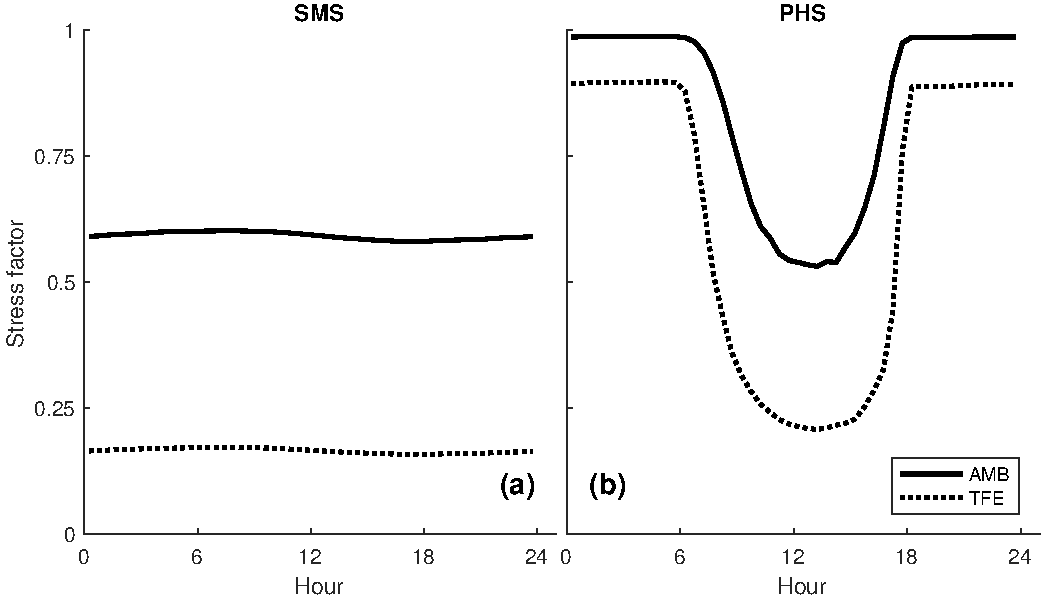
\includegraphics[width=30pc]{../figs3/fig4.pdf}
     \caption{2003 dry season (SON) diurnal mean water stress function for 
     (a) SMS, and
     (b) PHS.
     Note that the water stress factor equals 1 when there is no stress and 0 when fully stressed.
     }
     \label{fig:stress1}
  \end{figure}
  
      \clearpage
    \begin{figure}[h]
     \centering
     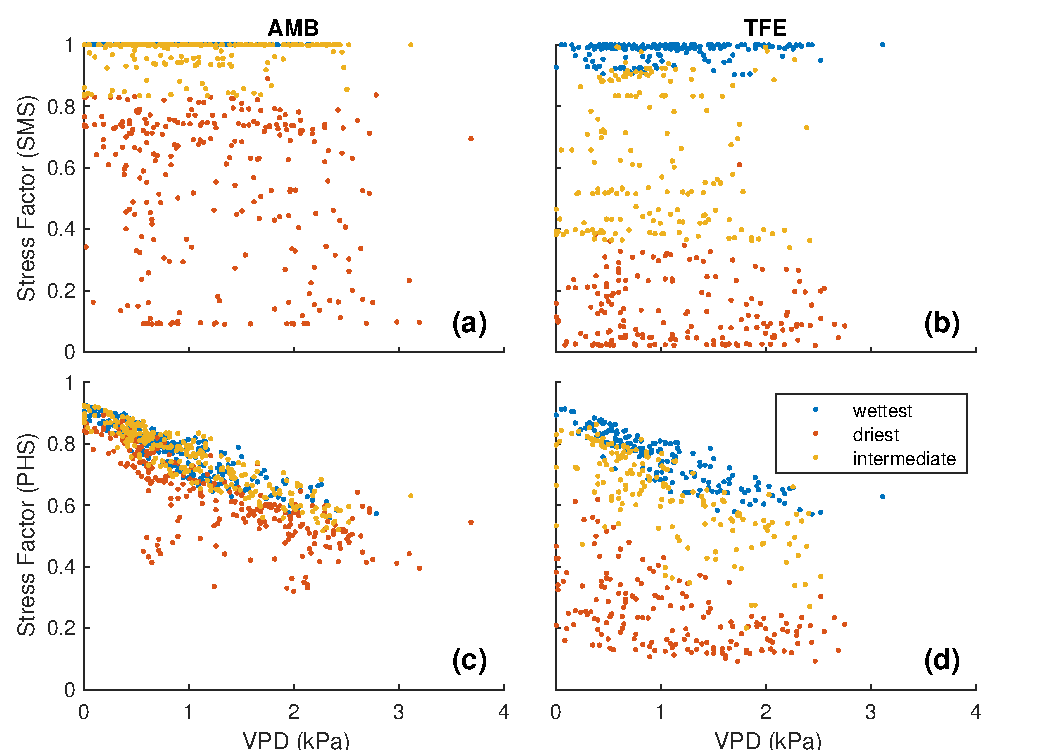
\includegraphics[width=30pc]{../figs3/vpdstress.pdf}
     \caption{Water stress factor versus vapor pressure deficit (2002-2003), constrained to timesteps with downwelling shortwave radiation between 400 and 425 W/m2 (n=515).
     Radiation is controlled to highlight the relationship with VPD, the reverse (controlling for VPD) is shown in Figure \ref{supp:fsds}.
     For SMS (a,b), data are subdivided based on average soil matric potential, weighted by root fraction.
     For PHS (c,d), data are subdivided based on predawn (5h) root water potential.
     Blue dots represent the wettest tercile, yellow dots represent the intermediate tercile, and red dots represent the driest tercile (values defining each tercile are in Table \ref{tab:tercile}).
     }
     \label{fig:stress2}
       \end{figure}
      
          \clearpage   
  \begin{figure}[h]
     \centering
     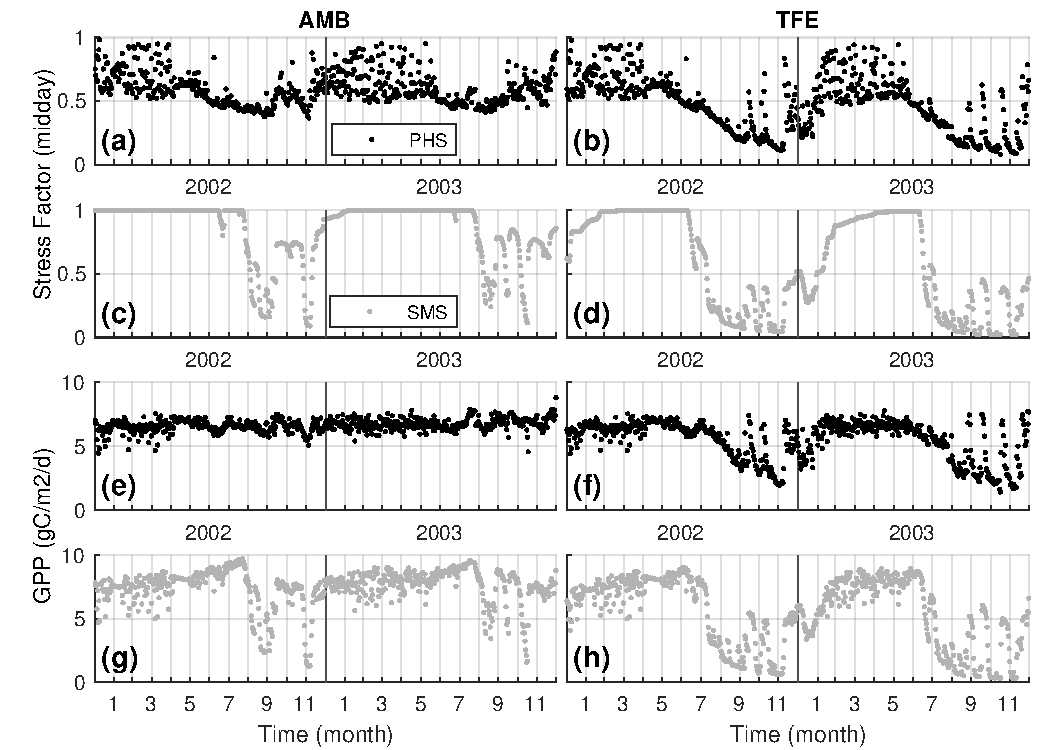
\includegraphics[width=30pc]{../figs3/gpp.pdf}
     \caption{(a-d) Daily stress factor (midday, averaged over 12h-14h) and (e-h) GPP (daily total) over 2002-2003 under ambient (left column) and TFE (right column) conditions.
     Output from the SMS configuration (a,b,e,f) are plotted with gray color, while output from the PHS configuration (c,d,g,h) are plotted in black.
     }
     \label{fig:gpp}
  \end{figure} 



      \clearpage
    \begin{figure}[h]
     \centering
     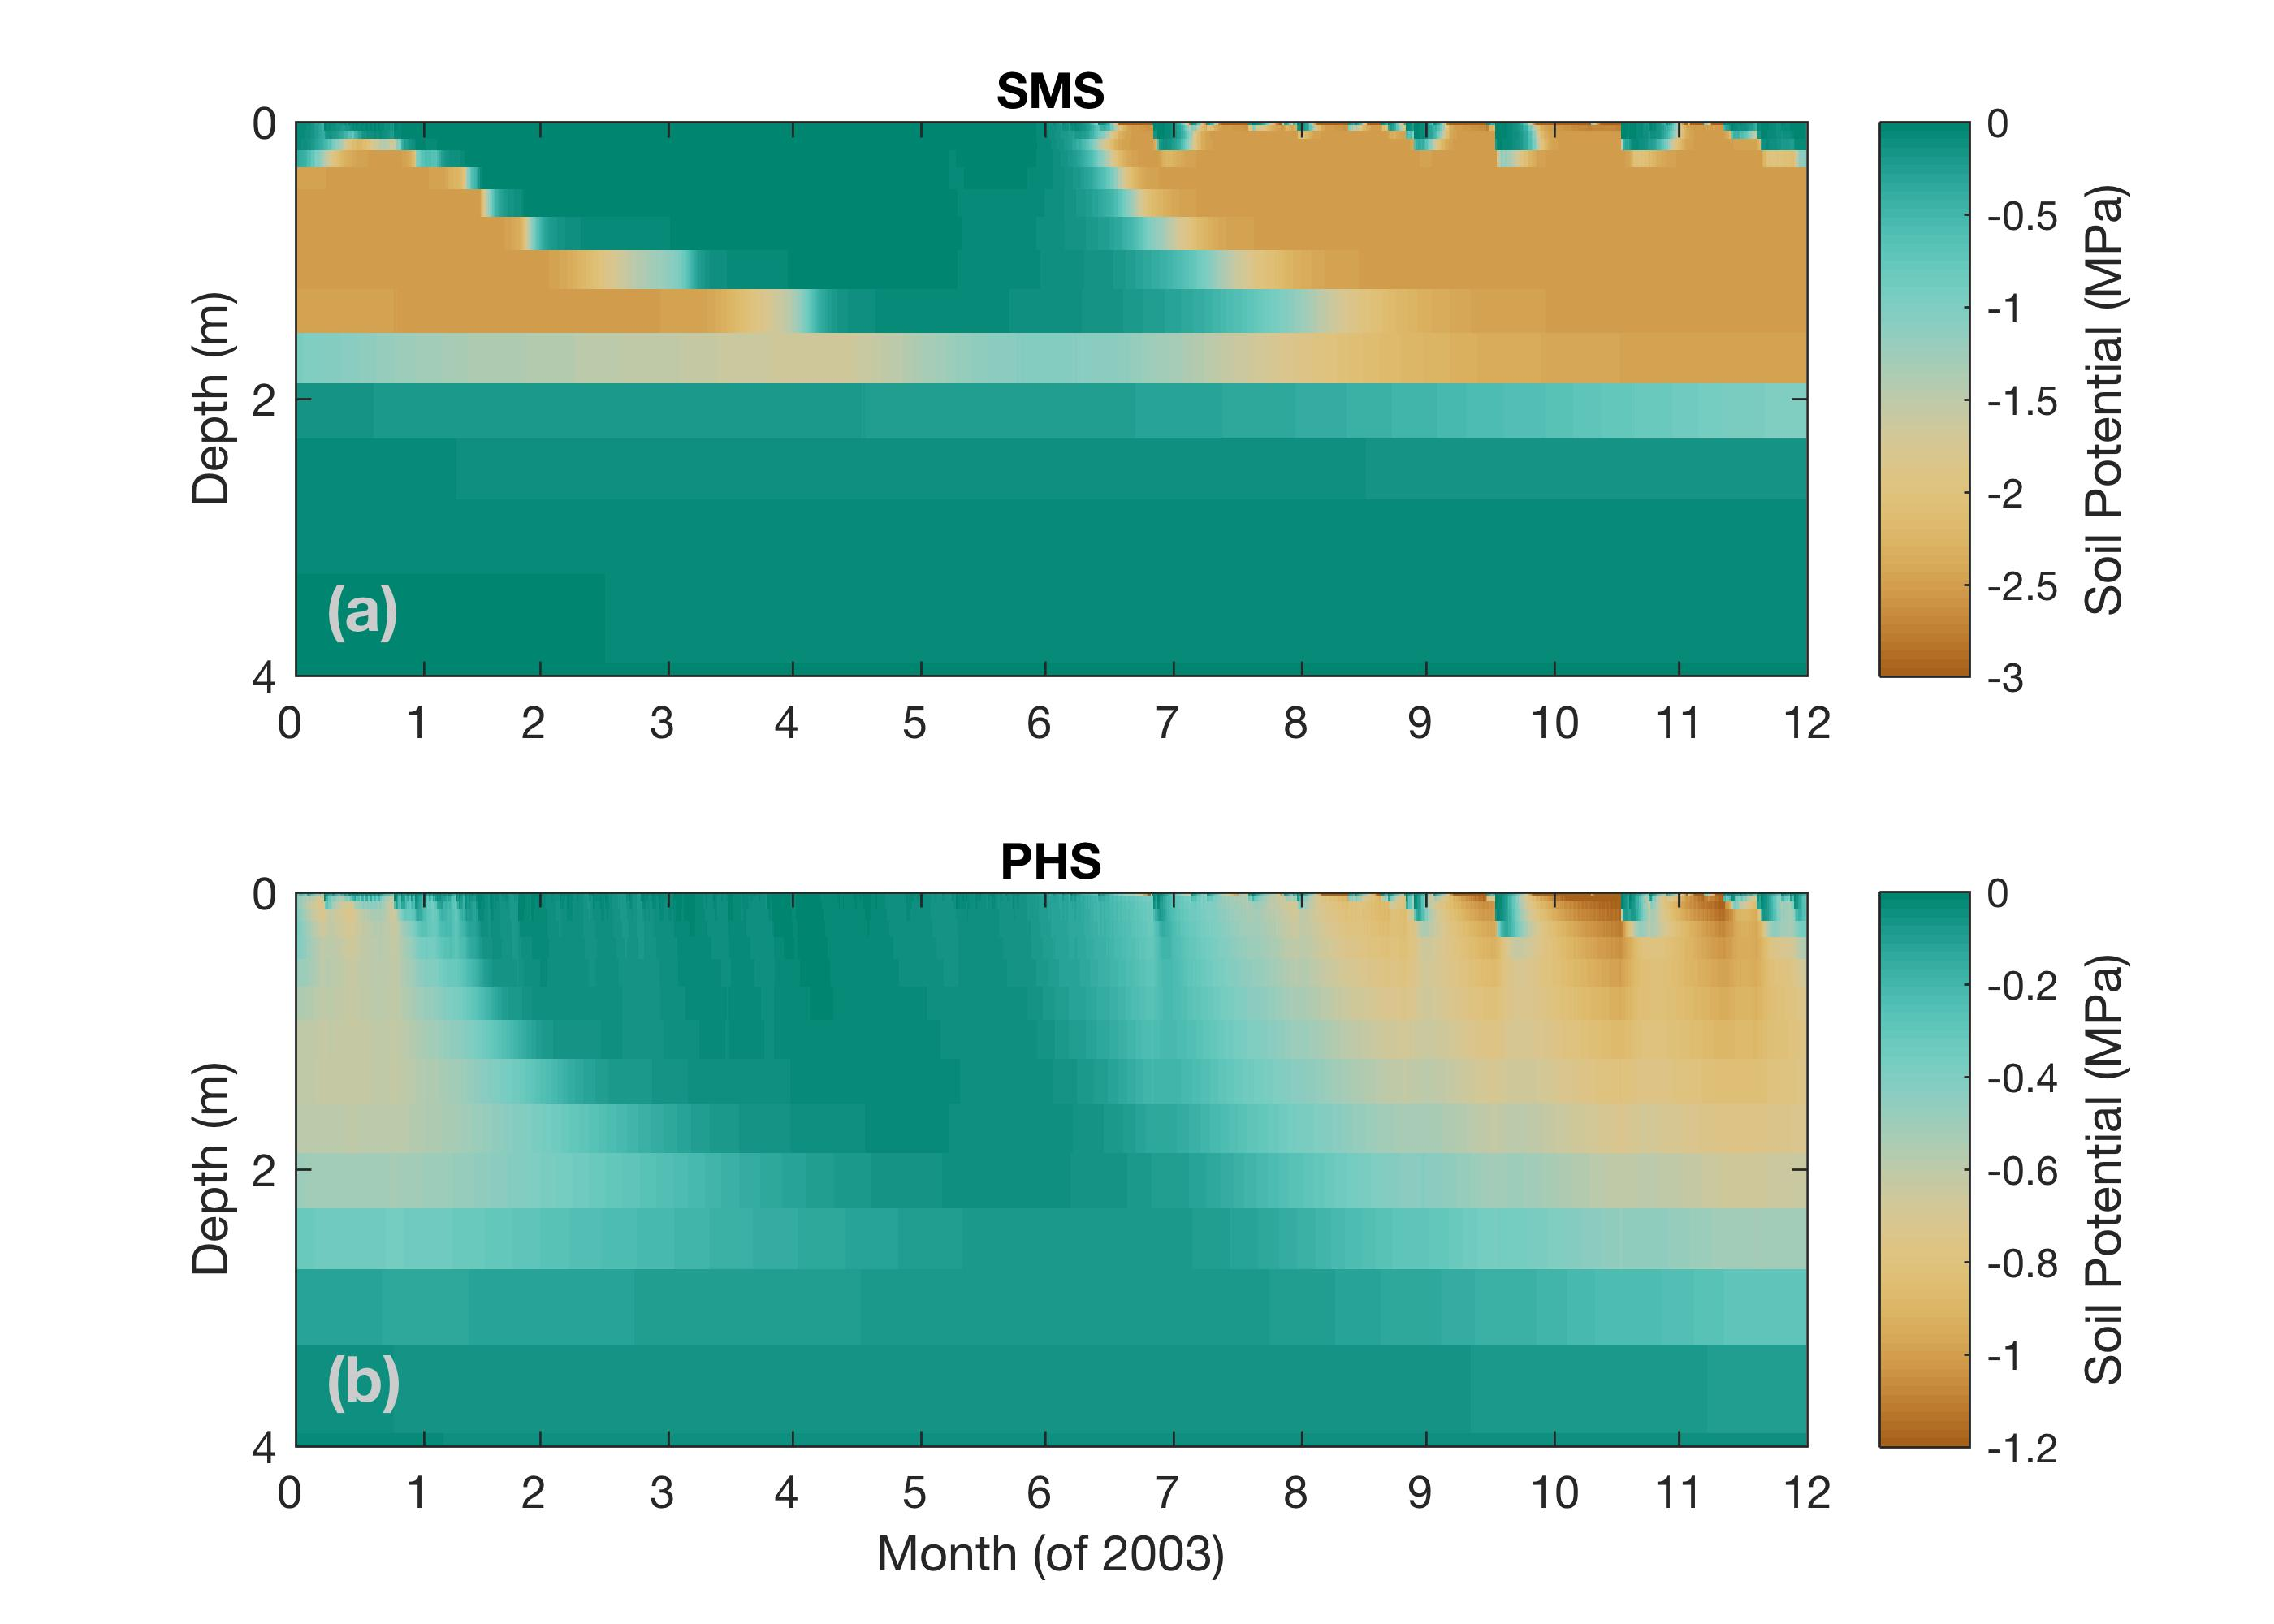
\includegraphics[width=30pc]{../figs3/smp.jpg}
     \caption{Vertical profile of soil water content (by volume) over 2003 under 60\% throughfall exclusion, for
     (a) SMS, and 
     (b) PHS.
     Soil water content under ambient conditions is shown in Supp Fig \ref{supp:sm}.
 }
     \label{fig:sm}
  \end{figure}

  \begin{figure}[h]
     \centering
     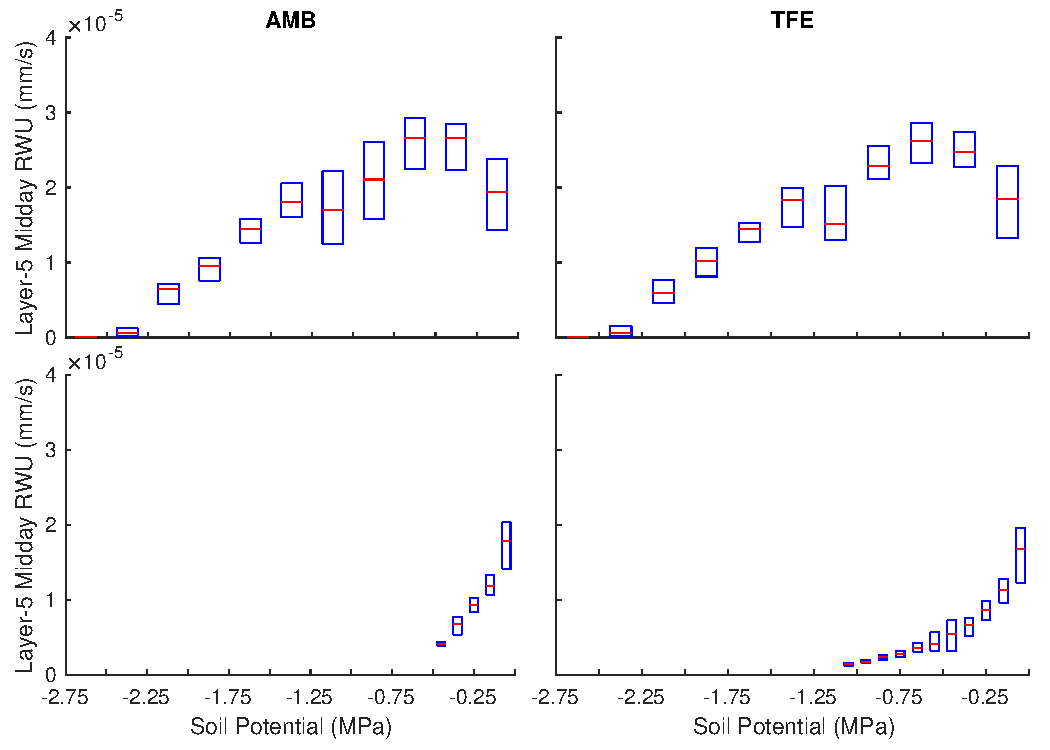
\includegraphics[width=30pc]{../figs3/rwu.pdf}
     \caption{Binned boxplot of root water uptake versus soil potential for Soil Layer 5 (2002-3).
     Red lines mark the median, with boxes spanning the interquartile range.
     Bin widths are 0.25 MPa for SMS and 0.1 MPa for PHS.
     Soil Layer 5 is shown, because it is close enough to the surface (20 to 32 cm) to experience a significant range in soil potential, and it has a large root fraction (14.4\%, only Soil Layer 6 has a larger root fraction).
     Only midday (12h-14h) timesteps are used to highlight the relationship with soil potential.}
     \label{fig:rwu}
  \end{figure}
  \clearpage

        \clearpage
    \begin{figure}[h]
     \centering
     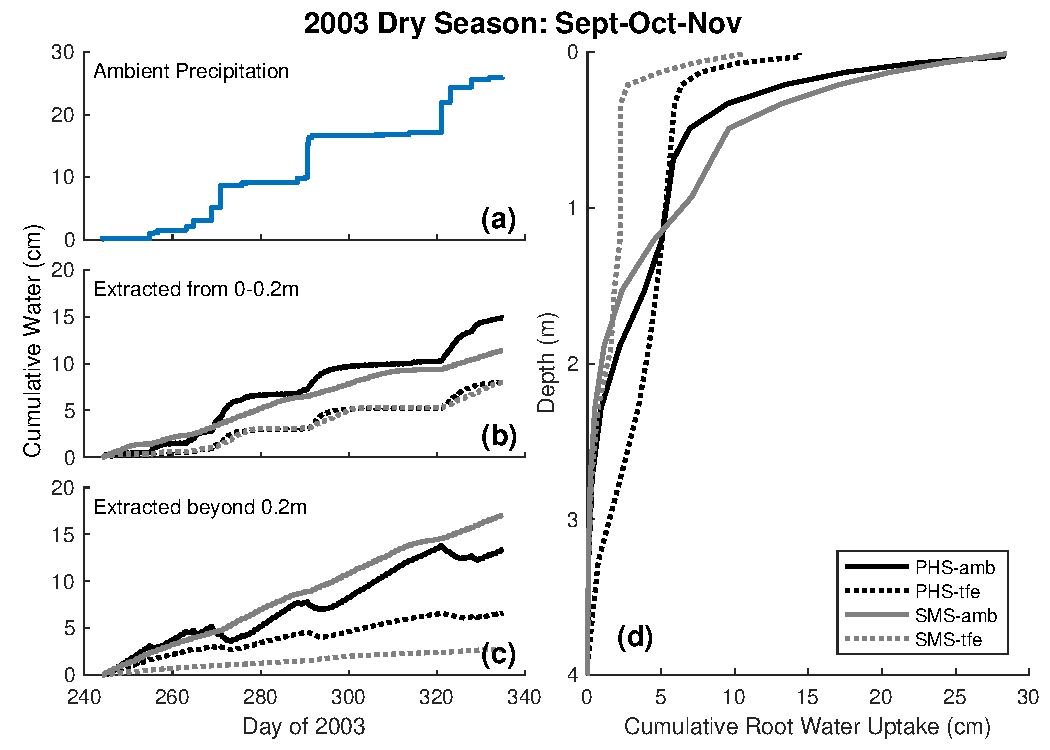
\includegraphics[width=30pc]{../figs3/qdry.pdf}
     \caption{2003 dry season (SON) cumulative root water uptake and precipitation. 
     (a) Cumulative precipitation over time under ambient conditions
     (b,c) Cumulative water uptake over time from above and below 0.2m, respectively.
     (d) Cumulative root water uptake over the soil column (accumulating from depth).
     }
     \label{fig:qdry}
  \end{figure}
               
    \clearpage
    \begin{figure}[h]
     \centering
     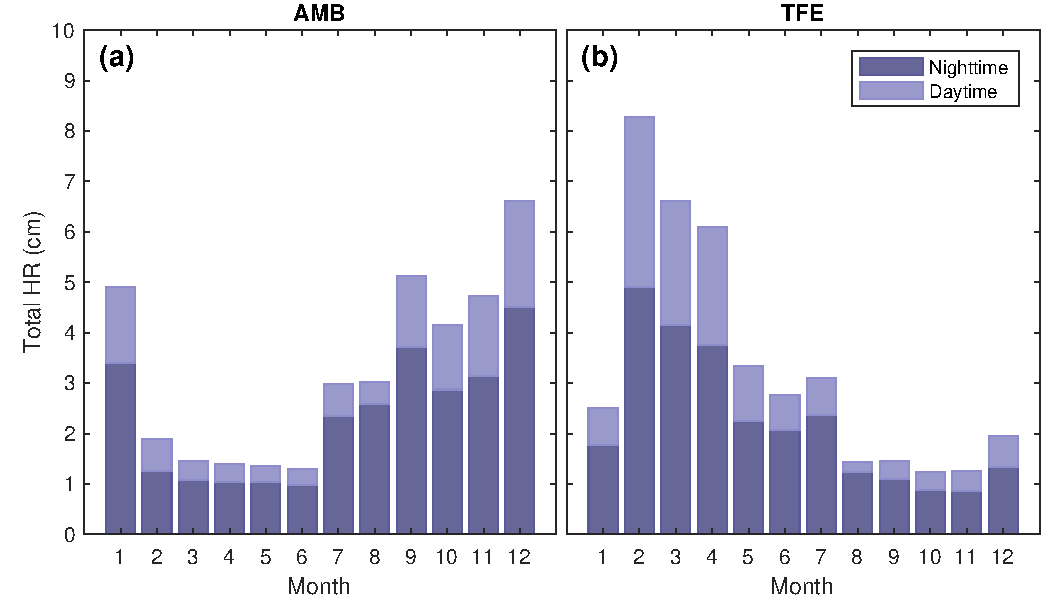
\includegraphics[width=30pc]{../figs3/hr.pdf}
     \caption{Total hydraulic redistribution (cm) by month across 2003. For (a) ambient through-fall conditions, and (b) 60\% throughfall exclusion. 
     Darker shading shows portion of HR at night [6pm,6am), lighter shading shows portion of HR during the day [6am,6pm).
     Total HR refers to the sum of all negative root water uptake flows, whenever water is deposited by roots into a given soil layer (instead of being extracted).}
     \label{fig:hr}
  \end{figure}

              \begin{figure}[h]
     \centering
     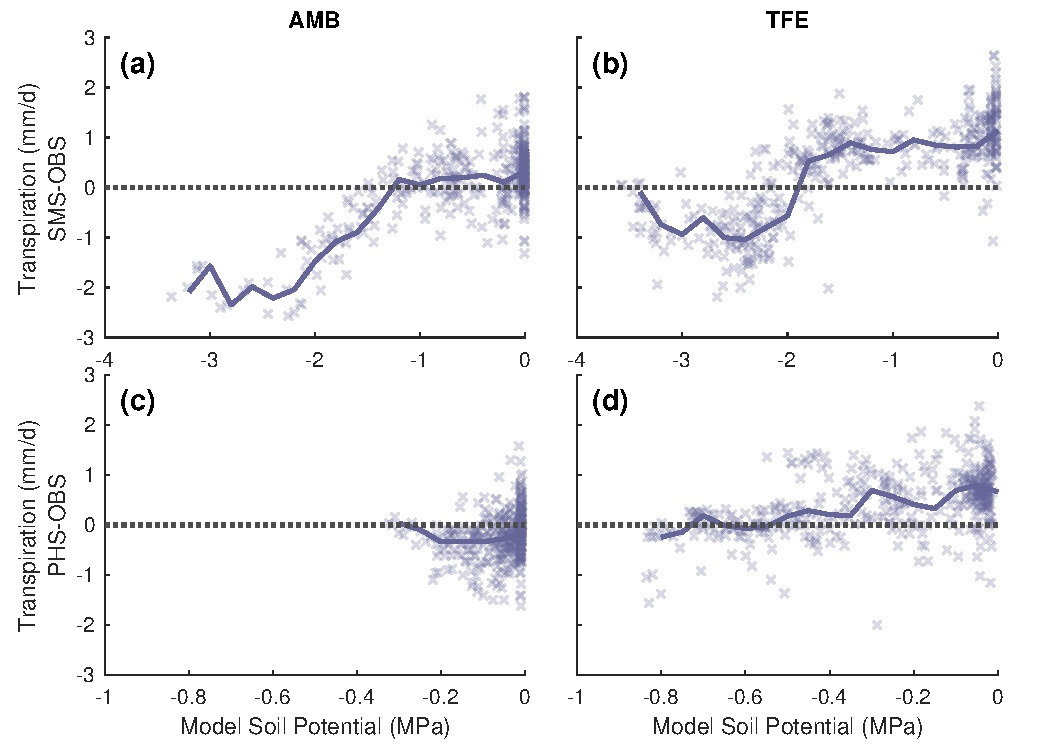
\includegraphics[width=30pc]{../figs3/t_err.pdf}
     \caption{Difference between modeled and observed transpiration (mm/d) versus model soil potential (MPa), for (a,b) SMS and (c,d) PHS.
     Solid lines are drawn at the median, binning points every 0.2MPa for SMS and 0.05 MPa for PHS (note the different soil potential axes). 
     Dotted lines are drawn at zero, where modeled and observed transpiration are in agreement.
     
     The two models use different root water uptake paradigms, from which we define different operators for column effective soil potential.
     For SMS we average over the soil column weighted by root fraction and over time (daily mean).
     For PHS we use predawn (5h) root water potential.
     Based on available observations, n = 414/436 days under ambient/TFE conditions.

}
     \label{fig:cool}
  \end{figure}
          \clearpage

\clearpage

\appendix
%====================
%  APPENDIX
%====================

\section{Supplementary Figures}


      \begin{figure}[h]
     \centering
     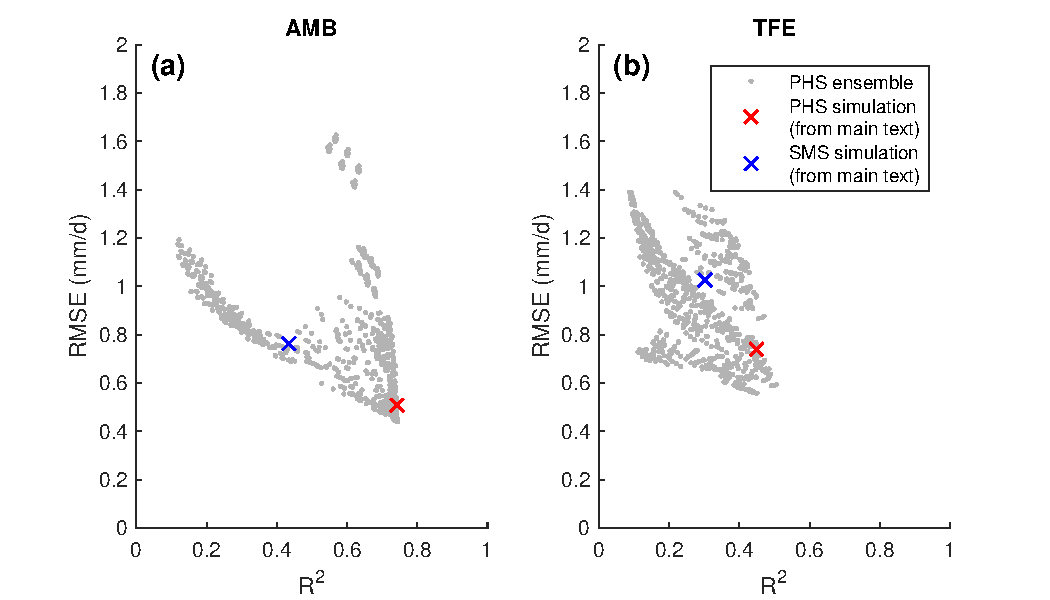
\includegraphics[width=30pc]{../figs3/ens.pdf}
     \caption{Parameter tuning exercise.
     }
     \label{supp:ens}
       \end{figure}
         \clearpage

        \clearpage

    \begin{figure}[h]
     \centering
     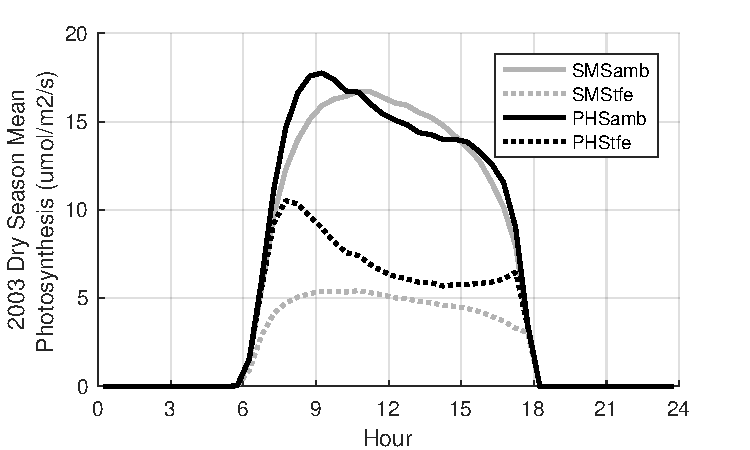
\includegraphics[width=20pc]{../figs3/suppfpsn.pdf}
     \caption{2003 dry season diurnal mean photosynthesis under ambient and TFE conditions for the two model configurations.
     }
     \label{supp:fpsn}
  \end{figure}


    \begin{figure}[h]
     \centering
     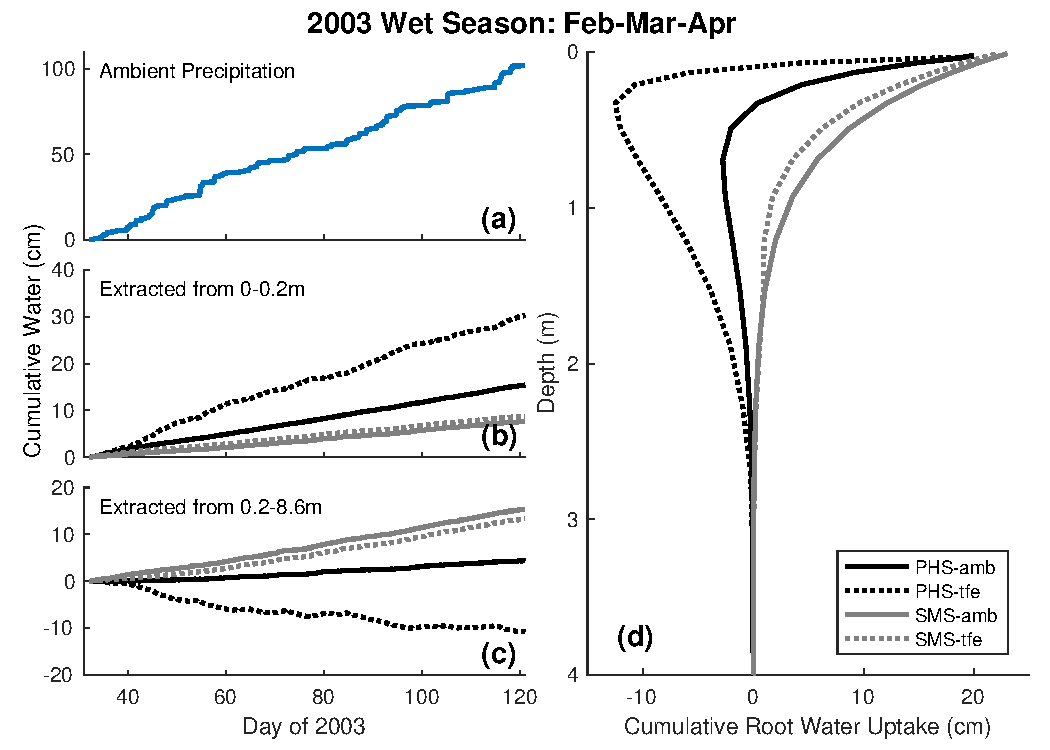
\includegraphics[width=30pc]{../figs3/qwet.pdf}
     \caption{2003 wet season (FMA) cumulative root water uptake and precipitation. 
     (a) Cumulative precipitation over time under ambient conditions
     (b,c) Cumulative water uptake over time from above and below 0.2m, respectively.
     (d) Cumulative root water uptake with depth.
     }
     \label{fig:qwet}
  \end{figure}


      \begin{figure}[h]
     \centering
     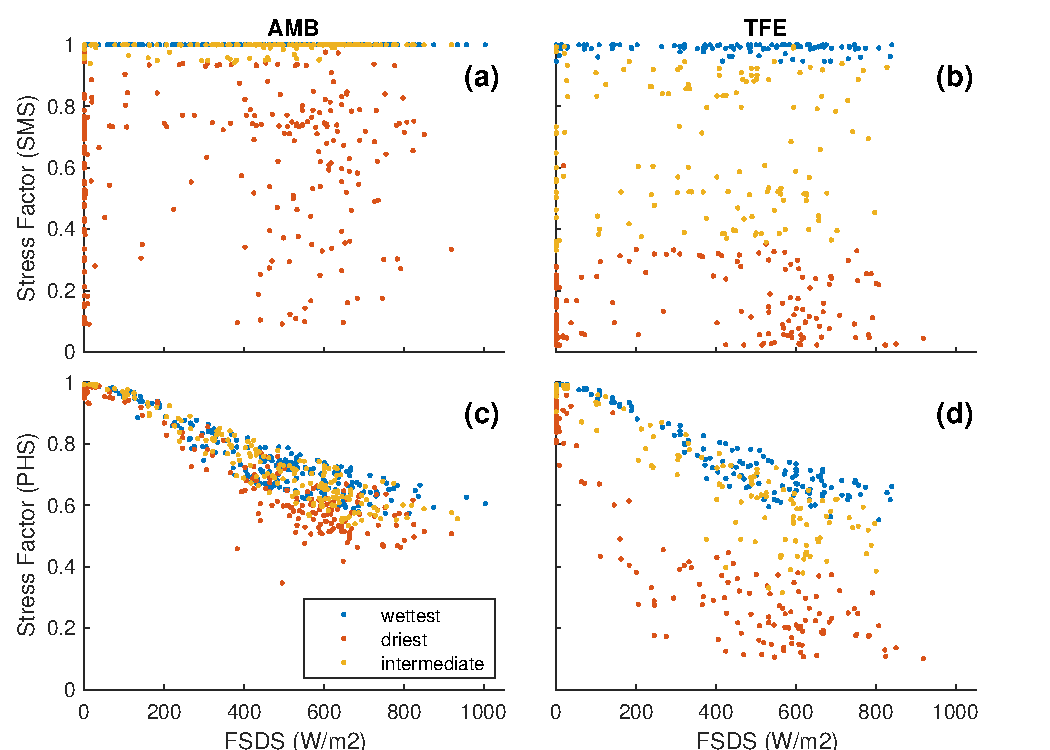
\includegraphics[width=30pc]{../figs3/suppstress.pdf}
     \caption{Water stress factor versus downwelling shortwave radiation (2002-2003), for timesteps with VPD between 1 and 1.0559 kPa (n=470).
     VPD is controlled to highlight the relationship with downwelling radiation, the reverse (controlling for radiation) is shown in Figure \ref{fig:stress2}.
     For SMS (a,b), data are subdivided based on average soil matric potential, weighted by root fraction.
     For PHS (c,d), data are subdivided based on predawn (5h) root water potential.
     Blue dots represent the wettest tercile, yellow dots represent the intermediate tercile, and red dots represent the driest tercile.
     }
     \label{supp:fsds}
       \end{figure}
         \clearpage

  \begin{figure}[h]
     \centering
     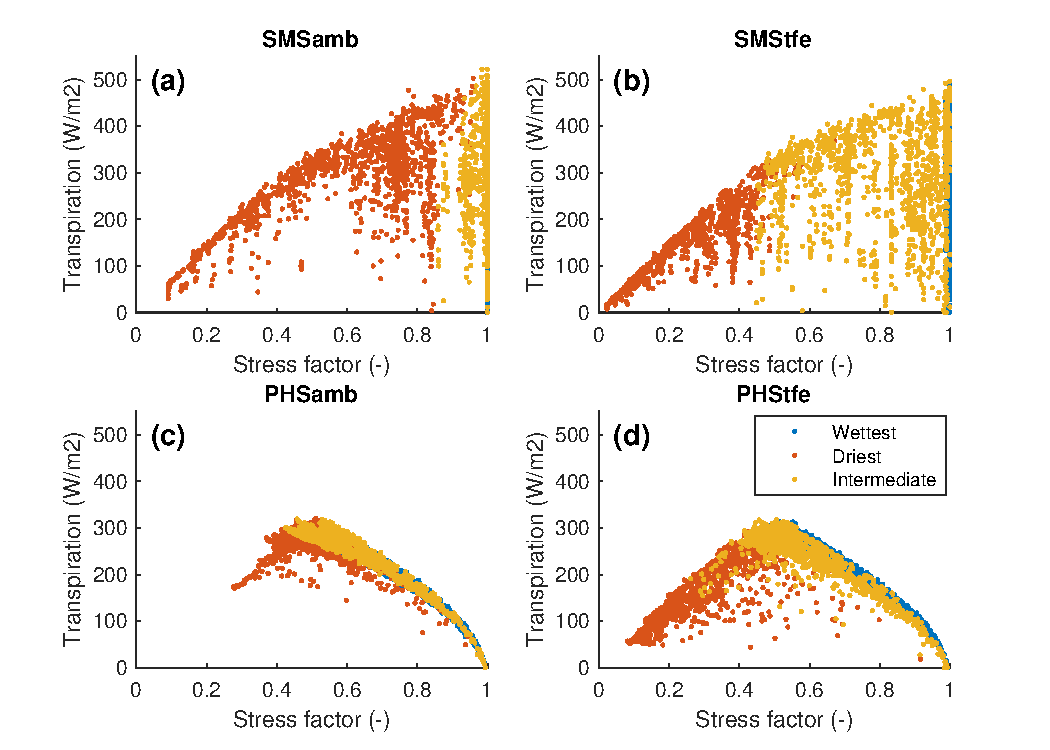
\includegraphics[width=30pc]{../figs3/supptstress.pdf}
     \caption{Midday transpiration vs. stress. 
     Data are colored by soil potential, subdivided into wettest, driest, and intermediate terciles.}
     \label{supp:tstress}
  \end{figure}
  \clearpage

  
  \begin{figure}[h]
     \centering
     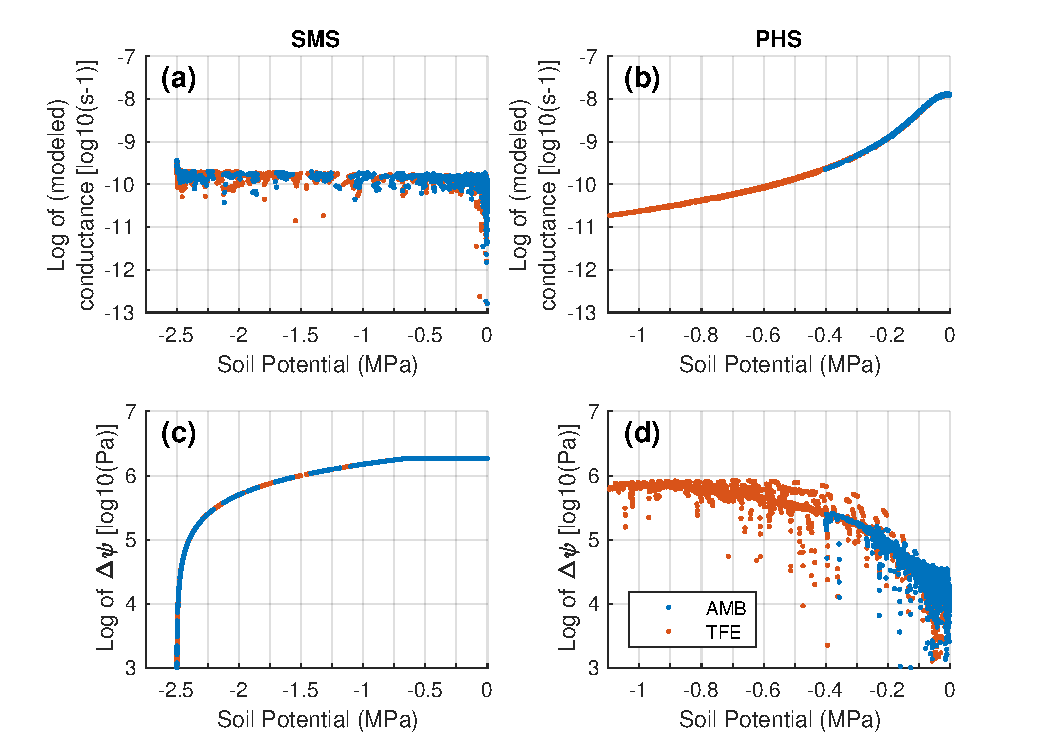
\includegraphics[width=30pc]{../figs3/suppcond.pdf}
     \caption{(a,b) Log of conductance ($k_{s,r}$) versus soil potential for Soil Layer 5.
     (c,d) Log of hydraulic gradient ($\Delta\psi$) versus soil potential for Soil Layer 5.
     Note that the soil potential axes vary for PHS vs. SMS. 
     
     Multiplied together $k_{s,r}$ and $\Delta\psi$ yield the Layer-5 root water uptake.
     PHS conductance decreases by almost 3 orders of magnitude between 0 and -1MPa, which leads to reduced RWU, though this is offset (by about half) due to increases in $\Delta\psi$.
     
     
     while SMS $\Delta\psi$ decreases by less than 1 order of magnitude between 0 and -2MPa, 
     leading to higher sensitivity to soil potential with PHS, see Figure \ref{fig:rwu}.
     
     Only midday (12h-14h, 2002-2003) timesteps are shown to emphasize the relationship with soil potential.
     With SMS, conductance is not modeled explicitly, but rather calculated as $k$=$q/\Delta\psi$ (see Section zqz). 
     For soil potentials greater than or equal to 2.5MPa, $\Delta\psi$=0, and SMS implied conductance is undefined, but could probably be considered to equal 0.
     PHS conductance captures both root tissue and soil matrix resistances (operating in series).}
     \label{supp:cond}
  \end{figure}
  \clearpage

\clearpage   
  \begin{figure}[h]
     \centering
     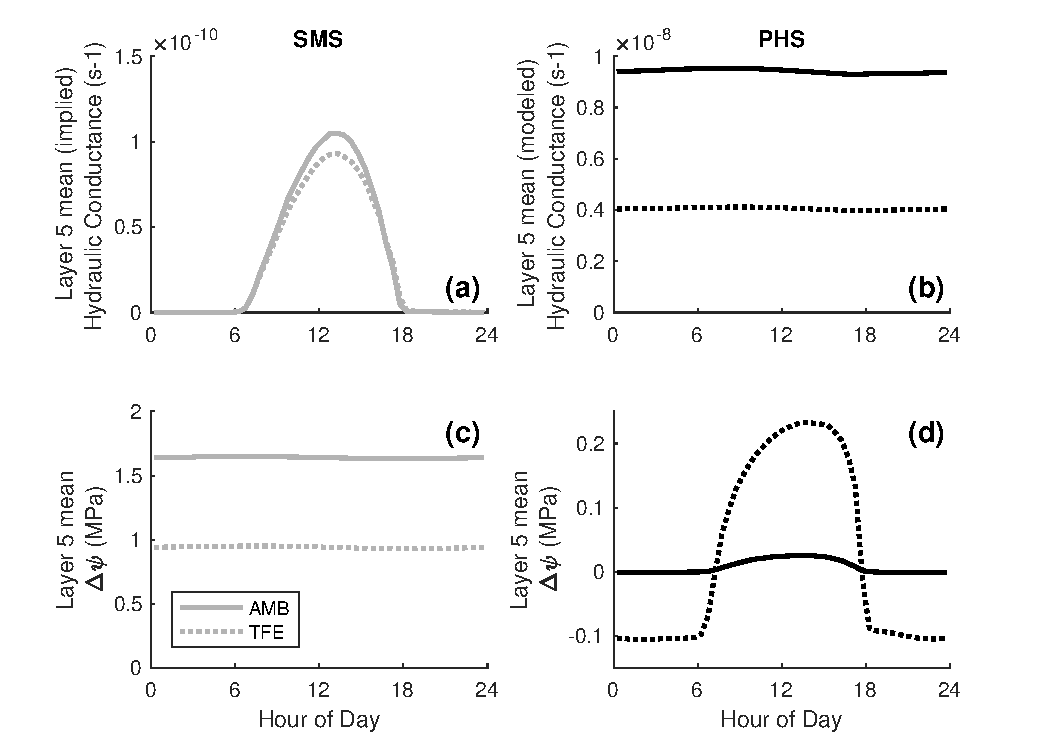
\includegraphics[width=30pc]{../figs3/k.pdf}
     \caption{2003 diurnal mean of Soil Layer 5 conductance and $\Delta\psi$, under ambient and TFE conditions. 
     }
     \label{supp:cond2}
  \end{figure}
  
      \begin{figure}[h]
     \centering
     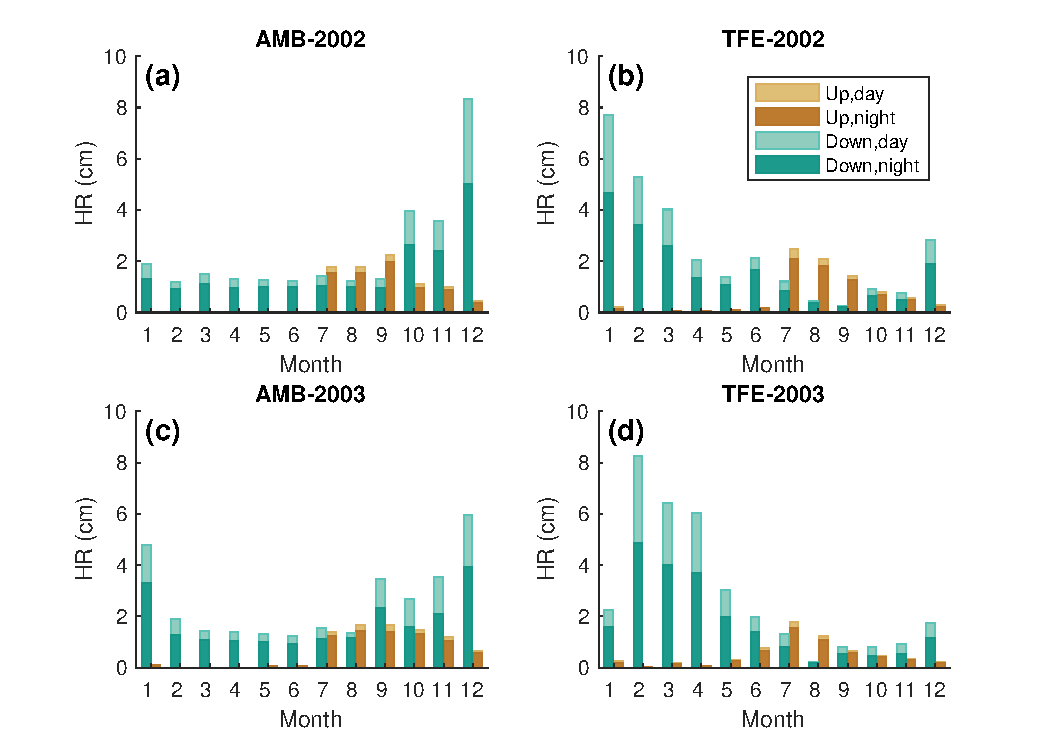
\includegraphics[width=30pc]{../figs3/hr2}
     \caption{PHS hydraulic distribution during 2003. Alternative version partitioning by direction.}
     \label{supp:hr}
  \end{figure}
  \clearpage

  
        \clearpage
    \begin{figure}[h]
     \centering
     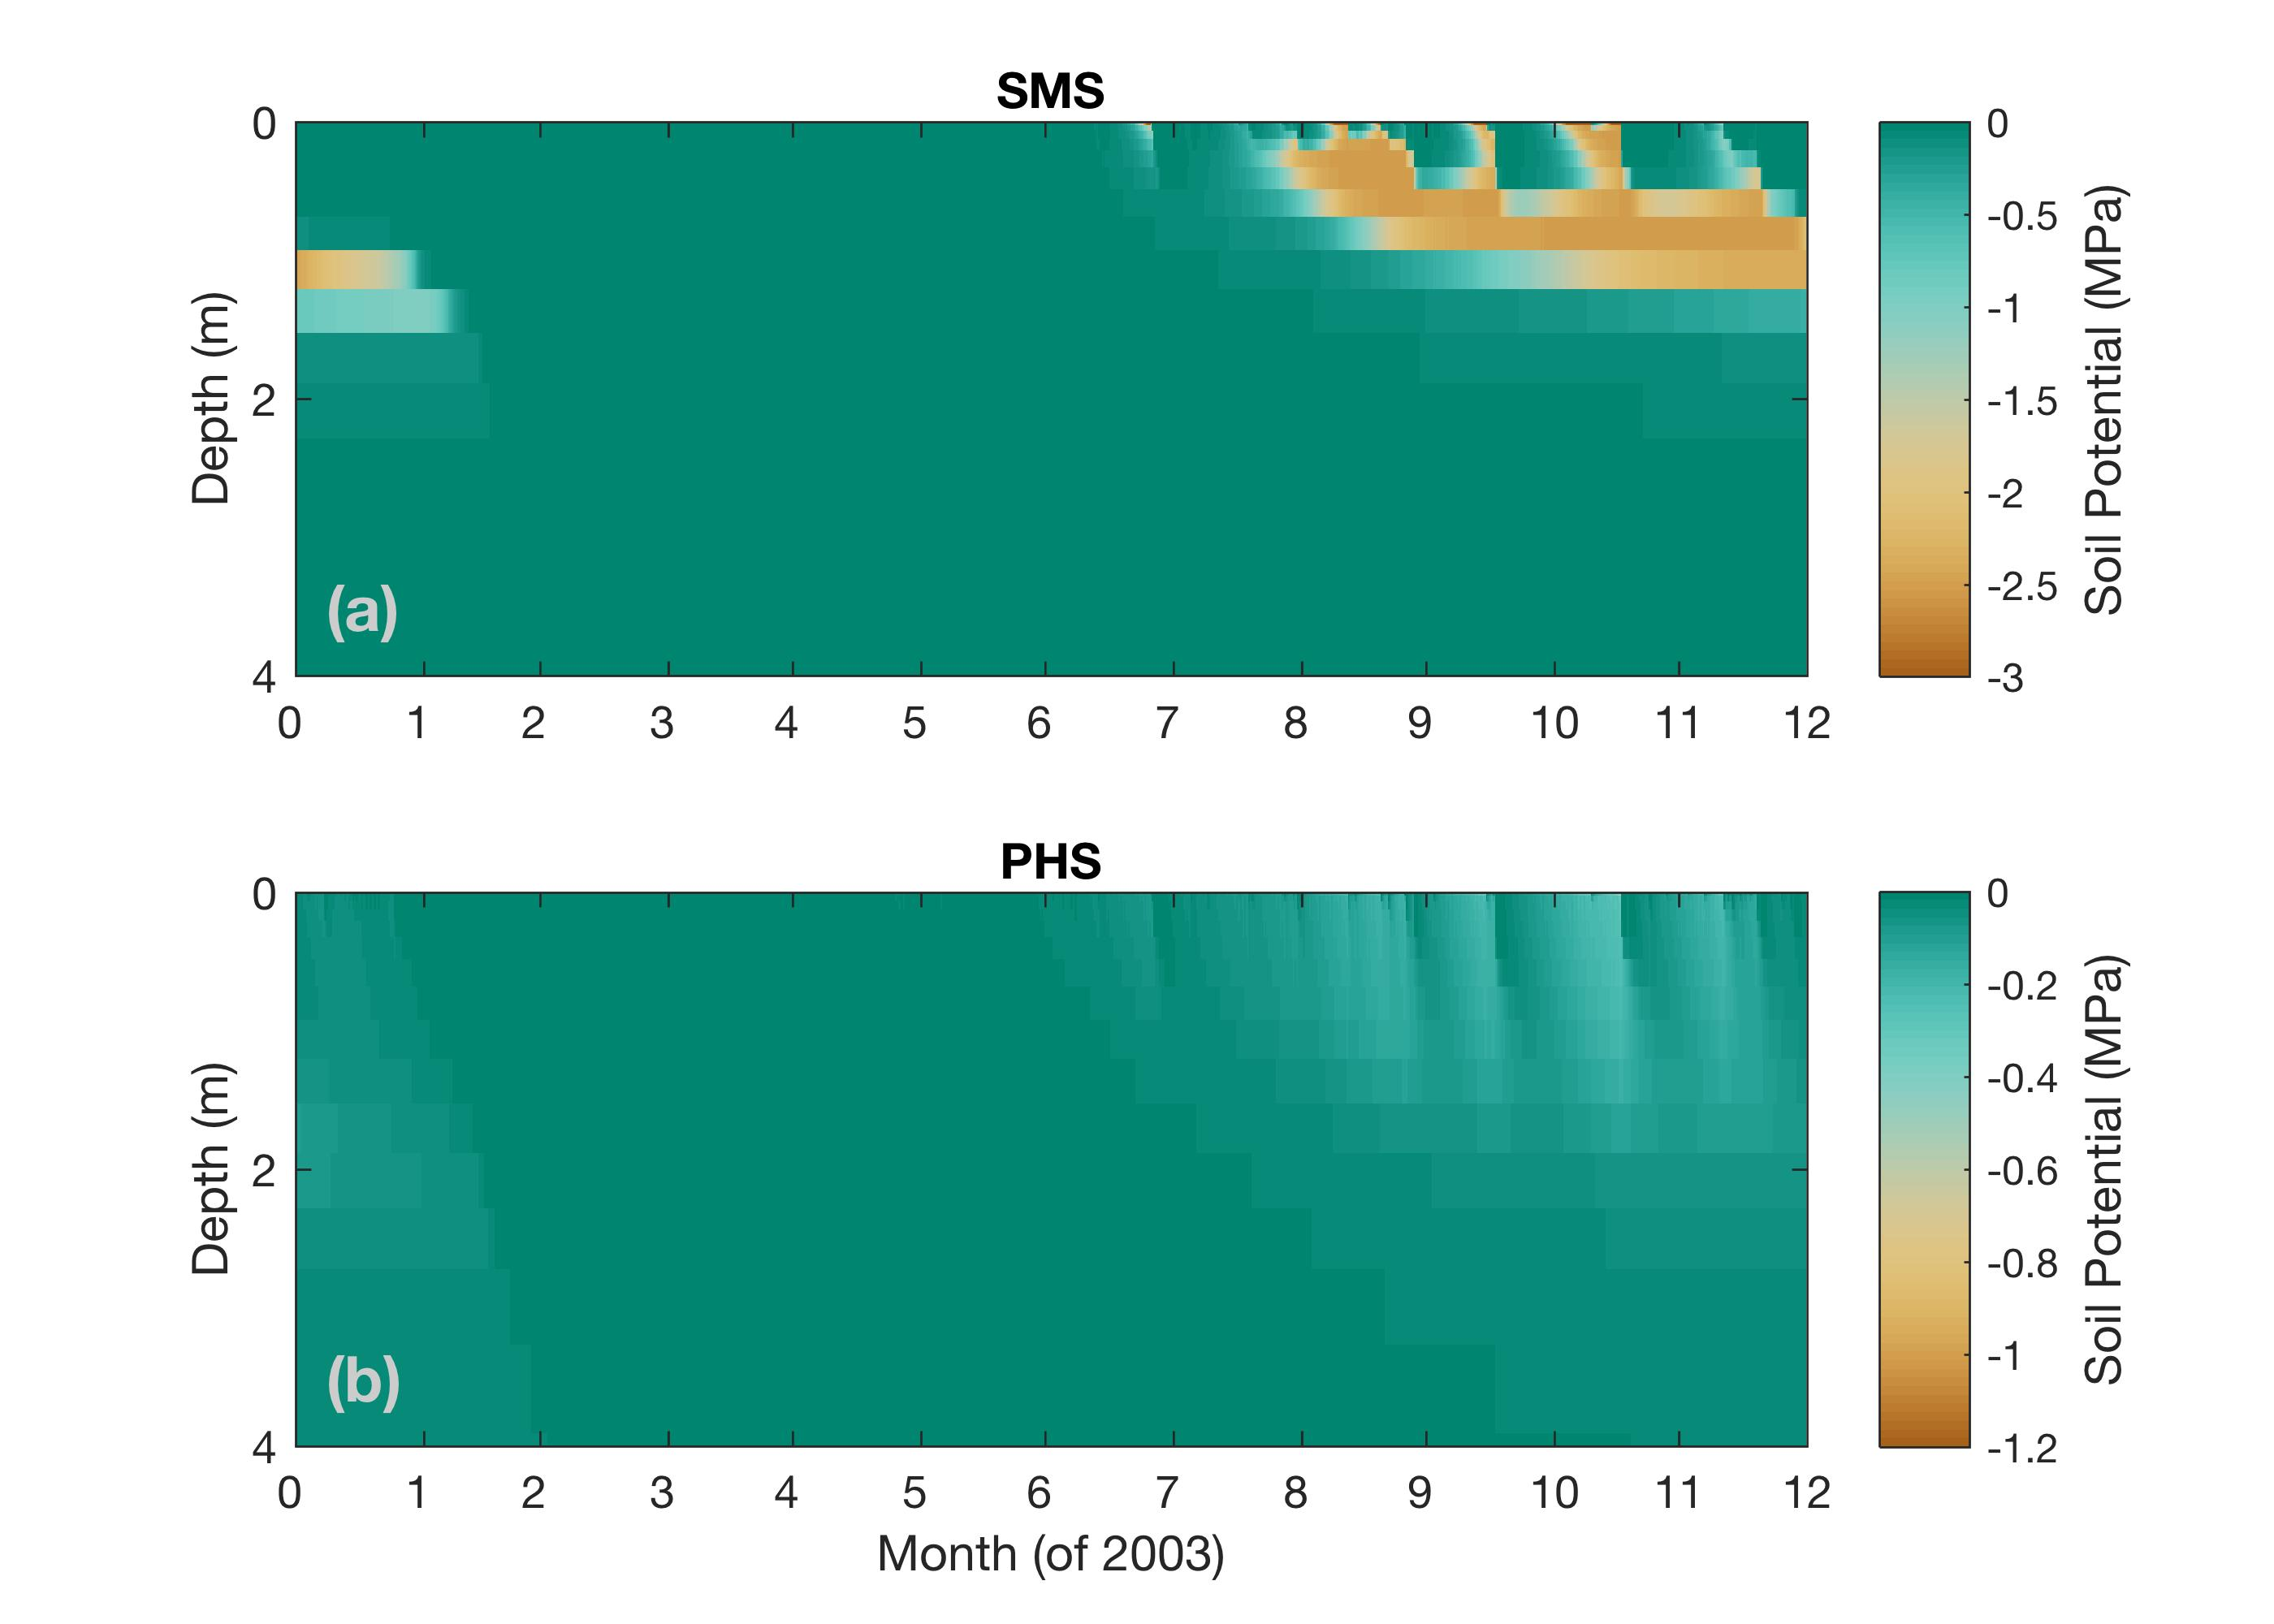
\includegraphics[width=30pc]{../figs3/suppsmp.jpg}
     \caption{Vertical profile of soil water content (by volume) through time under ambient through-fall conditions, for
     (a) PHS, and 
     (b) SMS. }
     \label{supp:sm}
  \end{figure}
  

    \begin{figure}[h]
     \centering
     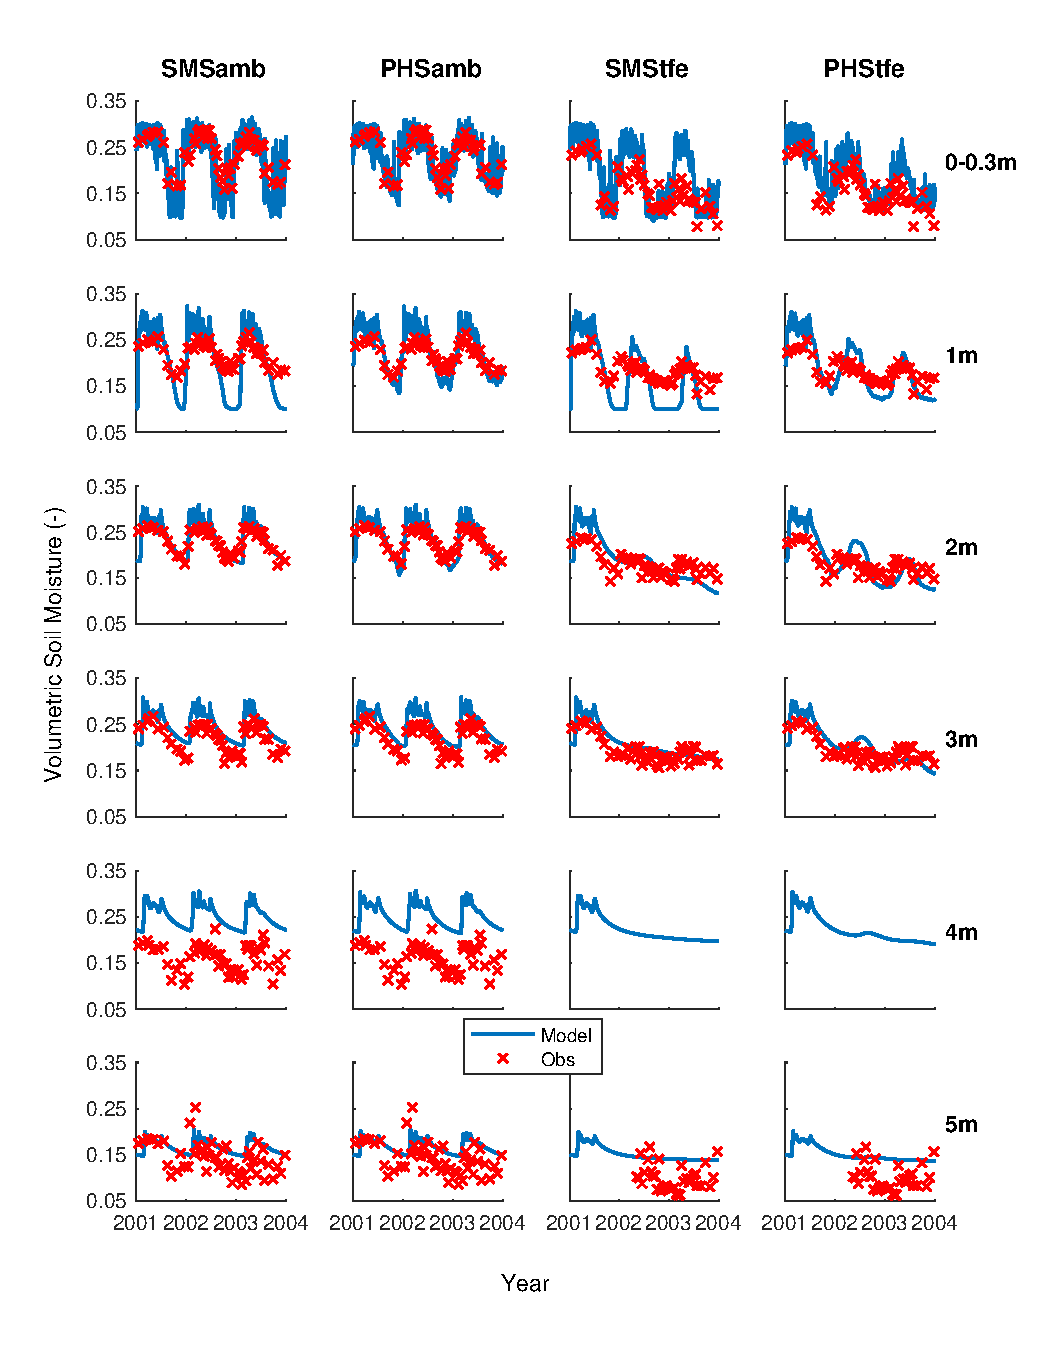
\includegraphics[width=30pc]{../figs3/suppsm2.pdf}
     \caption{Time series of soil moisture by soil layer.
     Complements Figure \ref{fig:sm}}
     \label{supp:sm2}
  \end{figure}
          \clearpage
          
     \begin{figure}[h]
     \centering
     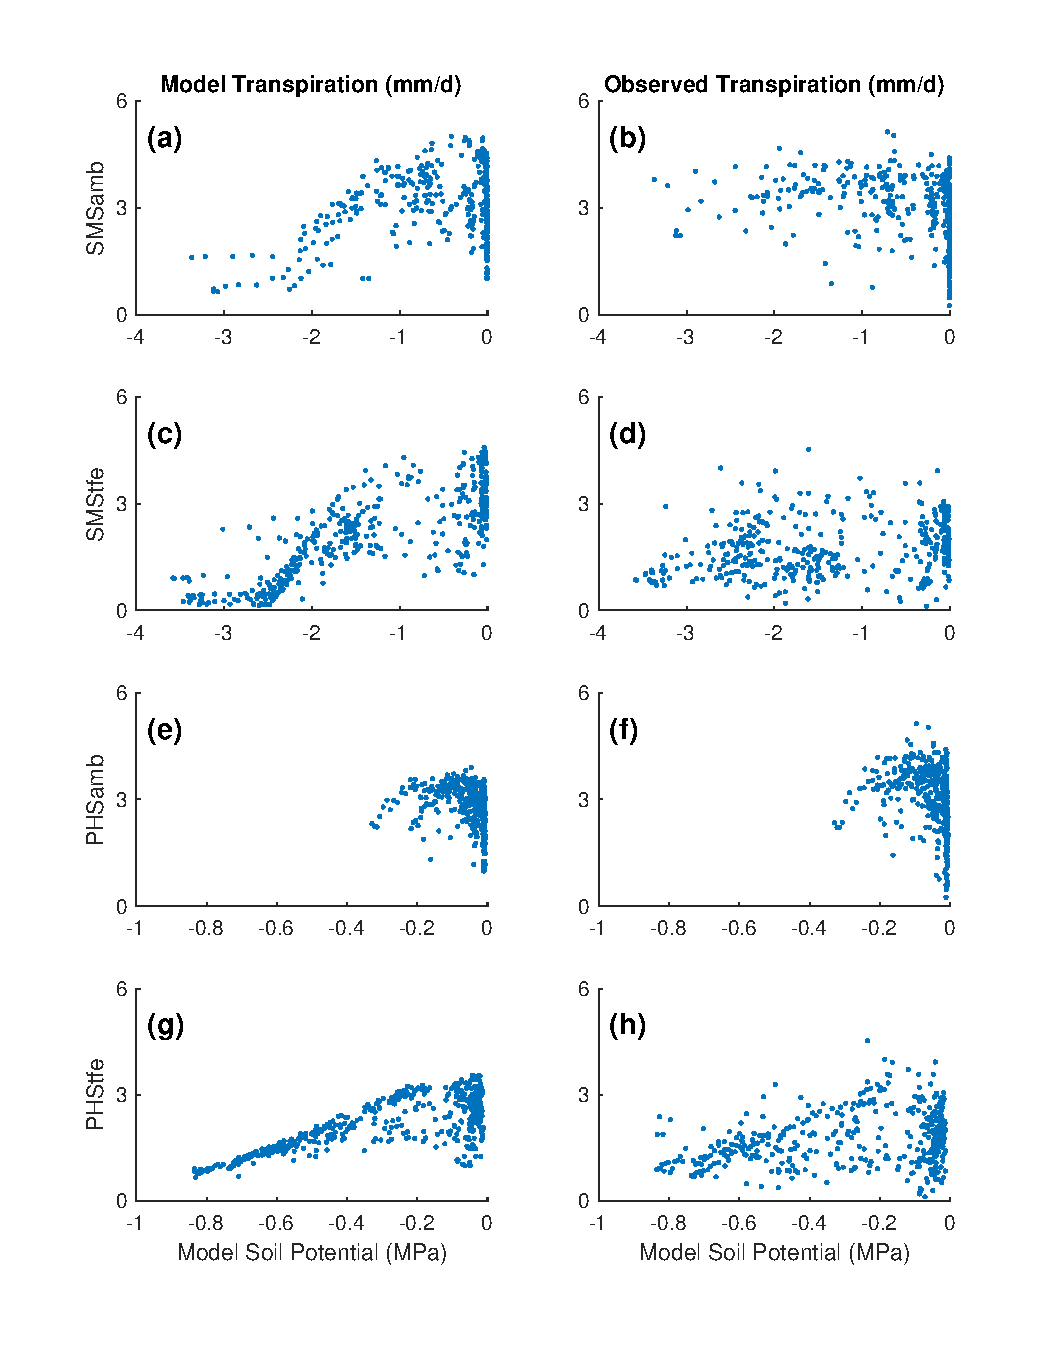
\includegraphics[width=30pc]{../figs3/suppcool.pdf}
     \caption{Modeled (left column) and observed (right column) transpiration  vs. model soil potential.
     Complements Figure \ref{fig:cool}}
     \label{supp:cool}
  \end{figure}
          \clearpage
          



\section{Appendix to Model Description}

% Details on water supply
\subsection{Details of Water Supply}

PHS resolves flow across four different segments, soil-to-root, root-to-stem, stem-to-leaf, and leaf-to-transpiration.

Stem-to-leaf. The area bases are sunlit and shaded leaf area, respectively. 
Note that gravity is assumed negligible here. 
Likewise there is no length scaling applied to maximum conductance. 
Therefore the input parameter for $k_{leaf,\text{max}}$ should be a conductance ($s^{-1}$).

\begin{linenomath*} \begin{equation} \begin{aligned}
q_{sun} &= k_{sun} \cdot \text{LAI-sun}  \cdot \left( \psi_{\text{stem}}-\psi_{\text{sun-leaf}}\right) \\
q_{shade} &= k_{shade} \cdot \text{LAI-shade} \cdot  \left( \psi_{\text{stem}}-\psi_{\text{shade-leaf}}\right)
\end{aligned} \end{equation} \end{linenomath*}

\begin{linenomath*} \begin{equation}
k_{sun} = k_{shade} = k_{leaf,\text{max}} \cdot f\left(\psi_{\text{stem}}\right)
\end{equation} \end{linenomath*}

\begin{linenomath*} \begin{equation} \begin{aligned}
f\left(\psi\right)=2^{-\left(\dfrac{\psi}{p_{50}}\right)^{c_k}}
\end{aligned} \end{equation} \end{linenomath*}

Root-to-stem. The area basis is stem area index. 
The input parameter is maximum stem xylem conductivity ($K_{stem,\text{max}}$).
Stem conductance ($k_{stem}$) is the result of scaling maximum conductivity by the tree height ($h$)
and applying loss relative to maximum conductance via the vulnerability curve $f\left(\psi_{\text{root}}\right)$. 
\begin{linenomath*} \begin{equation}
q_{stem} = k_{stem} \cdot  \text{SAI}  \cdot \left( \psi_{\text{root}}-\psi_{\text{stem}}-\rho g h\right)
\end{equation} \end{linenomath*}
\begin{linenomath*} \begin{equation}
k_{stem} = \dfrac{K_{stem,\text{max}}}{h} \cdot f\left(\psi_{\text{root}}\right)
\end{equation} \end{linenomath*}

Soil-to-root. Area basis is RAI in soil layer $i$, which is based on the layer root fraction times the
total root area. Total root area is calculated as the sum of stem and leaf area indices multiplied by a relative
root area parameter ($f_{\text{root}}$).
The vertical root distribution is defined by the layer root fraction ($r_i$), which follows a one-parameter 
(by PFT) power law decay following \citet{jackson1996}.

\begin{linenomath*} \begin{equation}
q_{sr,i} = k_{sr,i} \cdot  \text{RAI}_i  \cdot \left( \psi_{\text{soil,i}}-\psi_{\text{root}}-\rho g z_i\right)
\end{equation} \end{linenomath*}
\begin{linenomath*} \begin{equation}
\text{RAI}_i=f_{\text{root}} \cdot \left( \text{SAI} + \text{LAI} \right) \cdot r_i
\label{eq:rai}
\end{equation} \end{linenomath*}
\begin{linenomath*} \begin{equation}
k_{sr,i} = \dfrac{k_{r,i}+k_{s,i}}{k_{r,i}\cdot k_{s,i}}
\end{equation} \end{linenomath*}
\begin{linenomath*} \begin{equation}
k_{r,i} = \dfrac{K_{r,\text{max}}}{l_i} f \left(\psi_{\text{soil,i}}\right)
\end{equation} \end{linenomath*}
\begin{linenomath*} \begin{equation}
l_i = z_i + x
\end{equation} \end{linenomath*}
\begin{linenomath*} \begin{equation}
k_{s,i} = \dfrac{K_{s,i}}{d}
\end{equation} \end{linenomath*}

The soil-and-root conductance $k_{sr,i}$ reflects two resistors in series, from soil-to-root ($k_{s,i}$) and through the
root tissue ($k_{r,i}$).
The root tissue conductance is attenuated via the vulnerability curve framework. 
The input parameter is maximum root xylem conductivity, on the basis of RAI as defined above.
The root conductivity is scaled by the conducting length, which is estimated as the sum of soil layer depth ($z_i$)
and average lateral extent ($x$, static parameter).
The soil conductivity $K_{s,i}$ is calculated from the layer soil matric potential ($\psi_{soil,i}$) 
and soil properties as described in \citet{oleson2013} utilizing typical soil hydraulic theory \citep{brooks1964,clapp1978}.
The soil conductance ($k_{s,i}$) is the result of scaling the conductivity by $d$, 
 the distance between roots estimated following \citet{williams1996} and \citet{bonan2014}

% Details on water demand
\subsection{Details of Water Demand}

The CLM5 implementation utilizes the Medlyn stomatal conductance model \citep{medlyn2011}, while also applying water stress through $V_{\text{cmax}}$.
Transpiration is calculated reflecting contributions from both stomatal conductance and leaf boundary layer conductance ($g_b$).
    \begin{equation}
    \label{suppeq:vc}
    V_{\text{cmax}} = f_w\, V_{\text{cmax,ww}} 
    \end{equation}
    
    \begin{equation}
    \label{suppeq:gs}
    g_s=g_0+\left(1+\dfrac{g_1}{\sqrt{D}}\right)\dfrac{A}{C_a}
    \end{equation}
    
    \begin{equation}
    \begin{aligned}
    \label{suppeq:e1}
    E_{sun} &=   g_{s,sun}*\rho*\text{VPD}*lai_{sun}*\left(1+\dfrac{g_{s,sun}}{g_b}\right)^{-1} \\
    E_{shade} &=   g_{s,shade}*\rho*\text{VPD}*lai_{shade}*\left(1+\dfrac{g_{s,shade}}{g_b}\right)^{-1}
    \end{aligned}
    \end{equation}

At the beginning of a set of PHS iterations, we solve for $E_{\text{sun,max}}$ and $E_{\text{shade,max}}$, 
by running the stomatal conductance scheme with $f_w$ set to 1 (no stress).
Within each PHS iteration, we do not resolve the full stomatal conductance scheme, 
but instead consider only the linear attenuation of stomatal conductance by $f_w$.
Transpiration is attenuated relative to the maximal values according to leaf water potential.

    \begin{equation}
    \begin{aligned}
    \label{suppeq:e2}
    E_{\text{sun}} &=   E_{\text{sun,max}}*2^{-\left(\dfrac{\psi_{\text{leaf}}}{\psi_{50}}\right)^{c_k}} \\
    E_{\text{shade}} &=   E_{\text{shade,max}}*2^{-\left(\dfrac{\psi_{\text{leaf}}}{\psi_{50}}\right)^{c_k}}
    \end{aligned}
    \end{equation}
    
We define $f_w$ as the ratio of attenuated stomatal conductance ($g_{s,sun}$, $g_{s,shade}$) to maximal stomatal conductance ($g_{s,sun,max}$, $g_{s,shade,max}$),
where $g_{s,sun,max}$ and $g_{s,shade,max}$ are the stomatal conductance values associated with $E_{\text{sun,max}}$ and $E_{\text{shade,max}}$.
As such, the definition in the main text (Equation \ref{eq:d1}), represents a linear simplification between $f_w$, stomatal conductance, and transpiration.

    \begin{equation}
    \begin{aligned}
    \label{supp:fw}
    f_{w,sun} &= \dfrac{g_{s,sun}}{g_{s,sun,max}}    \\
    f_{w,shade} &= \dfrac{g_{s,shade}}{g_{s,shade,max}}
    \end{aligned}
    \end{equation}

After each PHS iteration, we compute $g_{s,sun}$ and $g_{s,shade}$ via Equations \ref{suppeq:vc} and \ref{suppeq:vc} (which involves iterating for intercellular $CO_2$ concentration).
We then update $g_{s,sun,max}$ and $g_{s,shade,max}$ to achieve consistency between equations (\ref{suppeq:e1}) and (\ref{suppeq:e2}).
At this point $g_{s,sun,max}$ and $g_{s,shade,max}$ no longer refer to the values associated with $f_w=1$, but rather also incorporate the non-linearity between $g_s$ and $f_w$.
The PHS iteration continues to convergence of $f_w$ (see Figure \ref{flowchart}).
The numerics have proven to be stable in practice, but future versions may aim to better integrate PHS within the stomatal conductance scheme to improve the coherence of Equations \ref{eq:d1} and \ref{supp:fw}.

    \begin{equation}
    \begin{aligned}
    g_{s,sun,max} &= \dfrac{g_{s,sun}}{f_{w,sun}} \\
    g_{s,shade,max} &= \dfrac{g_{s,shade}}{f_{w,shade}} \\
    \end{aligned}
    \end{equation}
    
         \begin{figure}[h]
     \centering
     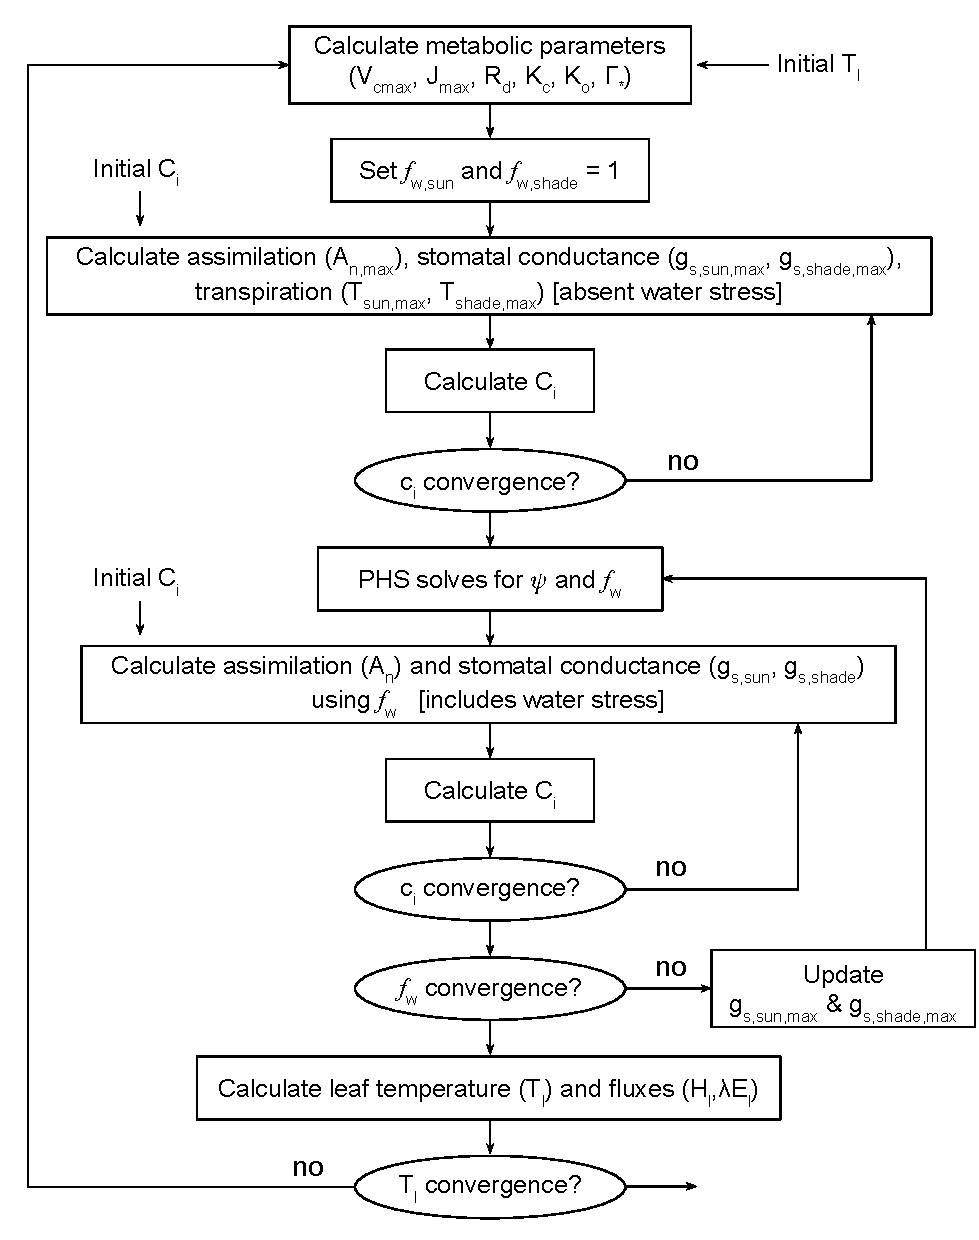
\includegraphics[width=30pc]{../figs3/schem3.pdf}
     \caption{Flow chart of PHS iterative solution}
     \label{flowchart}
  \end{figure}
          \clearpage

% Details on phs solution
\subsection{Details of Water Potential Solution}


The continuity of water flow through the system yields four equations
   \begin{linenomath*} \begin{equation}
   \begin{aligned}
   E_{sun}&=q_{sun}\\
   E_{shade}&=q_{shade}\\
   q_{sun}+q_{shade}&=q_{stem}\\
   q_{stem}&=\sum_{i=1}^{nlevsoi}{q_{sr,i}}
   \end{aligned}
   \end{equation} \end{linenomath*}

We seek the set of vegetation water potential values (four unknowns), 

   \begin{linenomath*} \begin{equation}
   \psi=\left[ \begin {array}{c} 
   \psi_{sunleaf}\cr\psi_{shadeleaf}\cr\psi_{stem}\cr\psi_{root}
   \end {array} \right] 
   \end{equation} \end{linenomath*}

that satisfies these equations, as forced by the soil moisture and atmospheric state. 

Each flux on the schematic can be represented in terms of the relevant water potentials. 

Defining the transpiration fluxes:


   \begin{linenomath*} \begin{equation}
   \begin{aligned}
   E_{sun} &= E_{sun,max} \cdot 2^{-\left(\dfrac{\psi_{sunleaf}}{p50}\right)^{c_k}} \\
   E_{shade} &= E_{shade,max} \cdot 2^{-\left(\dfrac{\psi_{shadeleaf}}{p50}\right)^{c_k}} 
   \end{aligned}
   \end{equation} \end{linenomath*}

Defining the water supply fluxes:

   \begin{linenomath*} \begin{equation}
   \begin{aligned}
   q_{sun}&=k_{leaf,max}\cdot 2^{-\left(\dfrac{\psi_{stem}}{p50}\right)^{c_k}} \cdot\mbox{LAI}_{sun}\cdot\left(\psi_{stem}-\psi_{sunleaf} \right) \\
   q_{shade}&=k_{leaf,max}\cdot 2^{-\left(\dfrac{\psi_{stem}}{p50}\right)^{c_k}}\cdot\mbox{LAI}_{shade}\cdot\left(\psi_{stem}-\psi_{shadeleaf} \right) \\
   q_{stem}&=\dfrac{k_{stem,max}}{z_2} \cdot 2^{-\left(\dfrac{\psi_{root}}{p50}\right)^{c_k}} \cdot SAI \cdot \left( \psi_{root} - \psi_{stem} - \Delta \psi_z  \right) \\
   q_{root}&=\sum_{i=1}^{nlevsoi}{q_{sr,i}}=\sum_{i=1}^{nlevsoi}{k_{sr,i}\cdot RAI\cdot\left(\psi_{soil,i}-\psi_{root} + \Delta\psi_{z,i} \right)}
   \end{aligned}
   \end{equation} \end{linenomath*}

In the CLM parameter file, $p50$ and $c_k$ are allowed to vary by flux level (transpiration vs. stem flux vs. root flux), but in our experiment (and on the default CLM parameter file), a single value is used for each.
PHS solves for the vector $\psi$
that satisfying water flow continuity as forced by atmospheric state and soil moisture.
Due to the model non-linearity, we use a linearized explicit approach, iterating with Newton's method. 
The initial guess is the solution for $\psi$ (vector) from the previous time step. 
The general framework, from iteration $m$ to $m+1$ is:

   \begin{linenomath*} \begin{equation} 
   \begin{aligned}
   q^{m+1}&=q^m+\dfrac{\delta q}{\delta\psi}\Delta\psi \\
   \psi^{m+1}&=\psi^{m}+\Delta\psi
   \end{aligned}
   \end{equation} \end{linenomath*}

So for our first flux balance equation, which requires sunlit leaf transpiration equal the flux of water from the main stem to the sunlit leaf, we have (at iteration $m+1$):

   \begin{linenomath*} \begin{equation} 
   E_{sun}^{m+1}=q_{sun}^{m+1}
   \end{equation} \end{linenomath*}

This can be linearized to:

   \begin{linenomath*} \begin{equation} 
   E_{sun}^{m}+\dfrac{\delta E_{sun}}{\delta\psi}\Delta\psi=q_{sun}^{m}+\dfrac{\delta q_{sun}}{\delta\psi}\Delta\psi
   \end{equation} \end{linenomath*}

And rearranged to be:

   \begin{linenomath*} \begin{equation} 
   \dfrac{\delta q_{sun}}{\delta\psi}\Delta\psi-\dfrac{\delta E_{sun}}{\delta\psi}\Delta\psi=E_{sun}^{m}-q_{sun}^{m}
   \end{equation} \end{linenomath*}

And for the other 3 flux balance equations:

   \begin{linenomath*} \begin{equation} 
   \begin{aligned}
   \dfrac{\delta q_{shade}}{\delta\psi}\Delta\psi-\dfrac{\delta E_{sha}}{\delta\psi}\Delta\psi&=E_{sha}^{m}-q_{1b}^{m} \\
   \dfrac{\delta q_{stem}}{\delta\psi}\Delta\psi-\dfrac{\delta q_{sun}}{\delta\psi}\Delta\psi-\dfrac{\delta q_{shade}}{\delta\psi}\Delta\psi&=q_{sun}^{m}+q_{shade}^{m}-q_{stem}^{m} \\
   \dfrac{\delta q_{soil}}{\delta\psi}\Delta\psi-\dfrac{\delta q_{stem}}{\delta\psi}\Delta\psi&=q_{stem}^{m}-q_{soil}^{m}
   \end{aligned}
   \end{equation} \end{linenomath*}

Putting all four together in matrix form:

   \begin{linenomath*} \begin{equation} 
   \left[ \begin {array}{c}
   \dfrac{\delta q_{1a}}{\delta\psi}-\dfrac{\delta E_{sun}}{\delta\psi} \cr
   \dfrac{\delta q_{1b}}{\delta\psi}-\dfrac{\delta E_{sha}}{\delta\psi} \cr
   \dfrac{\delta q_2}{\delta\psi}-\dfrac{\delta q_{1a}}{\delta\psi}-\dfrac{\delta q_{1b}}{\delta\psi} \cr
   \dfrac{\delta q_{soil}}{\delta\psi}-\dfrac{\delta q_2}{\delta\psi}
   \end {array} \right]
   \Delta\psi=
   \left[ \begin {array}{c}
   E_{sun}^{m}-q_{1a}^{m} \cr
   E_{sha}^{m}-q_{1b}^{m} \cr
   q_{1a}^{m}+q_{1b}^{m}-q_2^{m} \cr
   q_2^{m}-q_{soil}^{m}
   \end {array} \right]
   \end{equation} \end{linenomath*}

Now to expand the left-hand side, from vector $\psi$ to the four distinct plant water potential nodes, noting that many derivatives are zero (e.g. $\dfrac{\delta E_{sun}}{\delta\psi_{sha}}=0$)

Introducing the notation:
$A\Delta\psi=b$

   \begin{linenomath*} \begin{equation} 
   \Delta\psi=\left[ \begin {array}{c}
   \Delta\psi_{sunleaf} \cr
   \Delta\psi_{shadeleaf} \cr
   \Delta\psi_{stem} \cr
   \Delta\psi_{root}
   \end {array} \right] 
   \end{equation} \end{linenomath*}

   \begin{linenomath*} \begin{equation} 
   A=
   \left[ \begin {array}{cccc}
   \dfrac{\delta q_{1a}}{\delta \psi_{sun}}-\dfrac{\delta E_{sun}}{\delta \psi_{sun}}&0&\dfrac{\delta q_{1a}}{\delta \psi_{stem}}&0\cr
   0&\dfrac{\delta q_{1b}}{\delta \psi_{sha}}-\dfrac{\delta E_{sha}}{\delta \psi_{sha}}&\dfrac{\delta q_{1b}}{\delta \psi_{stem}}&0\cr
   -\dfrac{\delta q_{1a}}{\delta \psi_{sun}}&
   -\dfrac{\delta q_{1b}}{\delta \psi_{sha}}&
   \dfrac{\delta q_2}{\delta \psi_{stem}}-\dfrac{\delta q_{1a}}{\delta \psi_{stem}}-\dfrac{\delta q_{1b}}{\delta \psi_{stem}}&
   \dfrac{\delta q_2}{\delta \psi_{root}}\cr
   0&0&-\dfrac{\delta q_2}{\delta \psi_{stem}}&\dfrac{\delta q_{soil}}{\delta \psi_{root}}-\dfrac{\delta q_2}{\delta \psi_{root}}
   \end {array} \right]
   \end{equation} \end{linenomath*}

   \begin{linenomath*} \begin{equation} 
   b=
   \left[ \begin {array}{c}
   E_{sun}^{m}-q_{b1}^{m} \cr
   E_{sha}^{m}-q_{b2}^{m} \cr
   q_{b1}^{m}+q_{b2}^{m}-q_{stem}^{m} \cr
   q_{stem}^{m}-q_{soil}^{m}
   \end {array} \right]
   \end{equation} \end{linenomath*}

We can compute all the entries for $A$ and $b$ based on the soil potential and maximum transpiration forcings and can solve to find:

   \begin{linenomath*} \begin{equation} 
   \Delta\psi=A^{-1}b
   \end{equation} \end{linenomath*}

   \begin{linenomath*} \begin{equation} 
   \psi_{m+1}=\psi_m+\Delta\psi
   \end{equation} \end{linenomath*}

We iterate until $b\to 0$, signifying water flux balance through the system. The result is a final set of water potentials ( $\psi_{root}$, $\psi_{stem}$, $\psi_{shadeleaf}$, $\psi_{sunleaf}$) satisfying non-divergent water flux through the system. 

\subsection{Parameter tuning exercise}
\label{ens}

We used a factorial design to create 972 ensemble members based on the parameter values below.
We ran PHS simulations for each parameter vector under both AMB and TFE conditions.
All simulations used the same initial conditions, which were the result of a previous simulation.
We evaluated the ensemble members based on the fit to sap flux observations, selecting that which
 maximized $R^2_{amb}+R^2_{tfe}-RMSE_{amb}-RMSE_{tfe}$ (Supp Fig \ref{supp:ens}).

Stem conductivity, $k_{\text{max}}$: 2e-8, 4e-8, 8e-8 s$^{-1}$ \\
Root conductivity, $k_{\text{r,max}}$: 2e-9, 6e-8, 18e-9 s$^{-1}$ \\
Root and stem vulnerability $p_{50}$: -1.75, -2.25, -2.75 MPa \\
Stomatal $p_{50}$: above plus either 0 or 0.5MPa \\
Vulnerability shape parameter, $c_k$: 2.95, 3.95, 5.45 (unitless) \\
Medlyn slope, $g_1$: 6, 7 kPa$^{0.5}$ \\
Rooting depth parameter, $\beta$: 0.95, 0.98, 0.993 (unitless) 


\acknowledgments
 = enter acknowledgments here =

%====================
%   REFERENCES
%====================
\nocite{*} 
\bibliography{refs/all}


\listofchanges


\end{document}


